% E3 report for the supervisors. Built with `python paper/build.py --report e3` (paper/README.md).
% Content: a translation of paper/sections/e3_notes_fr.md (the author's notes), in their order. Where the notes and the
% repository disagreed on a fact listed in the Phase 0 review, the repository's version is written. Every number is a
% macro of ../numbers.tex, or is written as it is with a source comment and the num-ok marker.
\documentclass[10pt]{article}

\usepackage[T1]{fontenc}
\usepackage{lmodern}
\usepackage{amsmath}
\usepackage{amssymb}
\usepackage{graphicx}
\usepackage{booktabs}
\usepackage[numbers]{natbib}
\usepackage[textsize=scriptsize]{todonotes}
\setlength{\marginparwidth}{2.6cm}
\usepackage{hyperref}

\graphicspath{{../figures/out/}}

% Notation macros. One macro per symbol; the comment gives its name in the
% code (src/helplessness, experiments/E2_online_4zones/twin.py).
% Every macro is wrapped in \ensuremath, so it works in and out of math mode.

% Controllability I(a;s'|s), measures.controllability.controllability_from_tensor.
\newcommand{\MI}[3]{\ensuremath{I(#1;#2\mid #3)}}
% I_hat: controllability of the belief T_hat.
\newcommand{\Ihat}{\ensuremath{\hat{I}}}
% I_ref: controllability of the count-matched reference (not the analytic value).
\newcommand{\Iref}{\ensuremath{\hat{I}_{\mathrm{ref}}}}
% I_star: controllability of the true kernel P.
\newcommand{\Istar}{\ensuremath{I^{*}}}
% b = I_hat - I_ref.
\newcommand{\bhat}{\ensuremath{\hat{b}}}
% Believed transition kernel.
\newcommand{\That}{\ensuremath{\hat{T}}}
% True transition kernel.
\newcommand{\Ptrue}{\ensuremath{P}}
% Reference-environment kernel.
\newcommand{\Pref}{\ensuremath{P_{\mathrm{ref}}}}
% delta = V_star - V^{pi_hat}, the belief's policy evaluated under P.
\newcommand{\regret}{\ensuremath{\Delta}}
% l1: per-pair L1 error between T_hat and P.
\newcommand{\Lone}{\ensuremath{L_{1}}}
% Optimal value under P.
\newcommand{\Vstar}{\ensuremath{V^{*}}}
% Value under P of the policy derived from T_hat.
\newcommand{\Vpihat}{\ensuremath{V^{\hat{\pi}}}}
% Base-2 logarithm (written as a macro: its 2 is notation, not a number).
\newcommand{\logtwo}{\log_{2}}
% The null hypothesis of a test (written as a macro: its 0 is notation, not a number).
\newcommand{\Hnull}{\ensuremath{H_{0}}}
% R: the reward on arrival at the goal (E1's calibrated parameter).
\newcommand{\Rgoal}{\ensuremath{R}}
% Visit counts N(s,a).
\newcommand{\counts}{\ensuremath{N}}
% Paired online - matched difference of a quantity, e.g. \gap{\bhat}.
\newcommand{\gap}[1]{\ensuremath{#1^{\mathrm{on}} - #1^{\mathrm{m}}}}

% Reserved for E3.
% I_s: controllability of the decoded s-space kernel (E3 main measure).
\newcommand{\Is}{\ensuremath{\hat{I}_{s}}}
% I_z: controllability in latent space (E3 secondary measure).
\newcommand{\Iz}{\ensuremath{\hat{I}_{z}}}

% --- E3 (world model) ---------------------------------------------------------
% The name of E3's offline calibration condition (written as a macro: its 0 is a name, not a number).
% Robust: \nobreakdash breaks in moving arguments (captions, section titles).
\DeclareRobustCommand{\EThreeZero}{E3\nobreakdash-0}
% h_0: the RSSM's learned initial deterministic state (the canonical probe's context).
\newcommand{\hzero}{\ensuremath{h_{0}}}
% I_s projected on the 5 reachable successors (secondary measure).
\newcommand{\Isproj}{\ensuremath{\hat{I}_{s}^{\mathrm{proj}}}}
% alpha_app: position / appearance index of diagnostic D1.
\newcommand{\alphaapp}{\ensuremath{\alpha_{\mathrm{app}}}}
% alpha: weight of an action-independent component in the predicted kernel
% (campaign analysis; distinct from alpha_app and from E2's Dirichlet alpha).
\newcommand{\alphaind}{\ensuremath{\alpha}}
% K_s: decoded prior draws per (s, a) for the s-space kernel.
\newcommand{\Ks}{\ensuremath{K_{s}}}
% L1 errors of criterion C-b: world model and tabular twin, against P.
\newcommand{\LoneWM}{\ensuremath{L_{1}^{\mathrm{WM}}}}
\newcommand{\LoneB}{\ensuremath{L_{1}^{B}}}
% Off-support mass of a predicted kernel.
\newcommand{\offmass}{\ensuremath{m_{\mathrm{off}}}}
% p_goal: the goal head's probability that a latent state is the goal.
\newcommand{\pgoal}{\ensuremath{p_{\mathrm{goal}}}}
% KL weights: beta_dyn trains the prior only, beta_rep pulls the posterior.
\newcommand{\betadyn}{\ensuremath{\beta_{\mathrm{dyn}}}}
\newcommand{\betarep}{\ensuremath{\beta_{\mathrm{rep}}}}
% Jensen-Shannon divergence.
\newcommand{\JS}{\ensuremath{\mathrm{JS}}}
% The critic's value estimate.
\newcommand{\Vhat}{\ensuremath{\hat{V}}}
% The tabular twin (condition B).
\newcommand{\twin}{\ensuremath{B}}
% Names of the calibration criteria and diagnostics.
\DeclareRobustCommand{\Ca}{C\nobreakdash-a}
\DeclareRobustCommand{\Cb}{C\nobreakdash-b}
\DeclareRobustCommand{\Cc}{C\nobreakdash-c}
\newcommand{\DOne}{D1}
\newcommand{\DTwo}{D2}

% --- Pending values ------------------------------------------------------------
% A number or figure that depends on a batch not run yet (the E3 final campaign).
% Its argument (the macro or figure name) is not shown; numbers.tex writes it.
\newcommand{\pending}[1]{\textcolor{orange}{\textbf{[pending]}}}

% Generated by paper/numbers/gen_numbers.py -- never edit by hand.
% Generated by paper/numbers/gen_numbers.py -- do not edit by hand.
% Rerun `python paper/build.py --numbers` after any change to the results.

% src: experiments/E2_online_4zones/artifacts/figures/csv/F2_null_model_paired_diff.csv :: n_seeds (constant over rows quantity=b, zone=controllable_noisy)
\newcommand{\eTwoNSeeds}{20}
% src: experiments/E2_online_4zones/artifacts/figures/csv/F2_null_model_paired_diff.csv :: number of distinct checkpoint values (quantity=b, zone=controllable_noisy)
\newcommand{\eTwoNCheckpoints}{16}
% src: experiments/E2_online_4zones/artifacts/figures/csv/table3_budget_trend_power_law.csv :: n_points (quantity=b, zone=controllable_noisy)
\newcommand{\eTwoGapFitNPoints}{11}
% src: experiments/E2_online_4zones/artifacts/figures/csv/table3_budget_trend_power_law.csv :: exponent (quantity=b, zone=controllable_noisy)
\newcommand{\eTwoGapExponent}{\ensuremath{+0.005}}
% src: experiments/E2_online_4zones/artifacts/figures/csv/table3_budget_trend_power_law.csv :: exponent_bootstrap_ci95_low (quantity=b, zone=controllable_noisy)
\newcommand{\eTwoGapExponentCILow}{\ensuremath{-0.210}}
% src: experiments/E2_online_4zones/artifacts/figures/csv/table3_budget_trend_power_law.csv :: exponent_bootstrap_ci95_high (quantity=b, zone=controllable_noisy)
\newcommand{\eTwoGapExponentCIHigh}{\ensuremath{+0.274}}
% src: experiments/E2_online_4zones/artifacts/figures/csv/table1_paired_diff_by_zone.csv :: mean_diff (checkpoint=100000, zone=controllable_noisy, quantity=b): E2's online - matched gap on b in the CN zone, the effect E1 and E3 refer to
\newcommand{\eTwoEffectCN}{\ensuremath{-0.02}}
% src: configs/zones/e1_4zones.yaml :: grid_shape (square)
\newcommand{\eThreeGridSize}{12}
% src: configs/zones/e1_4zones.yaml :: blocks.*.rows / cols (side of every block)
\newcommand{\eThreeZoneSize}{5}
% src: configs/zones/e1_4zones.yaml :: number of blocks
\newcommand{\eThreeNZones}{4}
% src: src/helplessness/envs/dynamics/__init__.py :: N_ACTIONS
\newcommand{\eThreeNActions}{5}
% src: configs/zones/e1_4zones.yaml :: blocks.ne.p = blocks.se.p
\newcommand{\eThreeNoiseP}{0.125}
% src: configs/zones/e1_4zones.yaml :: 1 - p + p / N_ACTIONS (blocks.ne.p; envs/dynamics)
\newcommand{\eThreeNoiseMain}{0.9}
% src: configs/zones/e1_4zones.yaml :: p / N_ACTIONS (blocks.ne.p; envs/dynamics)
\newcommand{\eThreeNoiseMinor}{0.025}
% src: experiments/E3_worldmodel_4zones/config.yaml :: episode.goal_reward
\newcommand{\eThreeGoalReward}{\ensuremath{+50}}
% src: experiments/E3_worldmodel_4zones/config.yaml :: episode.step_reward
\newcommand{\eThreeStepReward}{\ensuremath{-1}}
% src: experiments/E3_worldmodel_4zones/config.yaml :: episode.max_steps
\newcommand{\eThreeEpisodeHorizon}{36}
% src: experiments/E3_worldmodel_4zones/config.yaml :: episode.gamma
\newcommand{\eThreeGamma}{0.9}
% src: experiments/E3_worldmodel_4zones/config.yaml :: episode.step_reward / (1 - episode.gamma)
\newcommand{\eThreeVNoGoal}{\ensuremath{-10}}
% src: configs/e3/gpu_campaign.yaml :: render.k
\newcommand{\eThreeRenderScale}{6}
% src: configs/e3/gpu_campaign.yaml :: render.cielab_marker_min_dist
\newcommand{\eThreeMarkerMinDist}{30}
% src: configs/e3/gpu_campaign.yaml :: model.n_vars
\newcommand{\eThreeLatentVars}{8}
% src: configs/e3/gpu_campaign.yaml :: model.n_classes
\newcommand{\eThreeLatentClasses}{8}
% src: configs/e3/gpu_campaign.yaml :: train.free_bits
\newcommand{\eThreeFreeBits}{0}
% src: configs/e3/gpu_campaign.yaml :: train.lr
\newcommand{\eThreeLr}{\ensuremath{10^{-3}}}
% src: configs/e3/gpu_campaign.yaml :: train.lr_after_switch
\newcommand{\eThreeLrAfterSwitch}{\ensuremath{10^{-4}}}
% src: configs/e3/gpu_campaign.yaml :: train.latent_estimator.switch_n_pairs
\newcommand{\eThreeSwitchPairs}{64}
% src: configs/e3/gpu_campaign.yaml :: train.latent_estimator.switch_eval_every
\newcommand{\eThreeSwitchEvalEvery}{50}
% src: configs/e3/gpu_campaign.yaml :: train.latent_estimator.switch_js_threshold
\newcommand{\eThreeSwitchJS}{3}
% src: configs/e3/gpu_campaign.yaml :: train.latent_estimator.switch_consecutive
\newcommand{\eThreeSwitchConsecutive}{5}
% src: configs/e3/gpu_campaign.yaml :: train.latent_estimator.collapse_js_threshold
\newcommand{\eThreeCollapseJS}{1}
% src: configs/e3/gpu_campaign.yaml :: train.batch_size
\newcommand{\eThreeBatchWindows}{16}
% src: configs/e3/gpu_campaign.yaml :: train.seq_len
\newcommand{\eThreeWindowLength}{64}
% src: configs/e3/gpu_e30b_win64.yaml :: train.batch_size x train.seq_len
\newcommand{\eThreeFramesPerUpdate}{1024}
% src: configs/e3/gpu_e30b_win16.yaml :: train.batch_size
\newcommand{\eThreeShortBatchWindows}{64}
% src: configs/e3/gpu_e30b_win16.yaml :: train.seq_len
\newcommand{\eThreeShortWindowLength}{16}
% src: configs/e3/gpu_campaign.yaml :: train.replay_ratio
\newcommand{\eThreeReplayRatio}{0.6}
% src: configs/e3/agent_mini.yaml :: train.replay_ratio
\newcommand{\eThreeReplayRatioMini}{2}
% src: configs/e3/gpu_campaign.yaml :: agent.epsilon
\newcommand{\eThreeEpsilon}{0.1}
% src: configs/e3/gpu_e30.yaml :: collection.epsilon
\newcommand{\eThreeEpsilonOffline}{1}
% src: configs/e3/gpu_campaign.yaml :: agent.k_act
\newcommand{\eThreeKAct}{16}
% src: configs/e3/gpu_campaign.yaml :: agent.horizon
\newcommand{\eThreeImagHorizon}{15}
% src: results/E3_worldmodel_4zones/*gpu_pilot_closed_loop__seed{00,05}*/meta.yaml :: agent.tie_tol_abs (the 4 runs agree)
\newcommand{\eThreeTieTol}{0.0751}
% src: configs/e3/gpu_campaign.yaml :: measure.kernel_k_s (= real_context.kernel_draws; checked against measures.kernel_probe.draws_for_l1_floor(CN kernel, 0.02))
\newcommand{\eThreeKs}{1358}
% src: results/E3_worldmodel_4zones/*gpu_e30b_win64__seed00* (experimental) arrays.npz P_true :: max over the CN rows of measures.kernel_probe.expected_l1_sampling_floor(row, 32)
\newcommand{\eThreeFloorOldK}{0.13}
% src: configs/e3/gpu_campaign.yaml :: measure.real_context.burn_in
\newcommand{\eThreeContextBurnIn}{8}
% src: configs/e3/gpu_pilot_closed_loop.yaml :: measure.real_context.max_per_state
\newcommand{\eThreeContextsPilot}{50}
% src: configs/e3/gpu_campaign.yaml :: measure.real_context.max_per_state
\newcommand{\eThreeContextsFinal}{200}
% src: configs/e3/gpu_campaign.yaml :: measure.iz_mc_samples_training
\newcommand{\eThreeIzMcTraining}{2000}
% src: configs/e3/gpu_campaign.yaml :: measure.iz_mc_samples_final
\newcommand{\eThreeIzMcFinal}{4096}
% src: configs/e3/gpu_pilot_closed_loop.yaml :: measure.checkpoint_goal_kernel.draws
\newcommand{\eThreeGoalDrawsPilot}{256}
% src: configs/e3/gpu_campaign.yaml :: measure.checkpoint_goal_kernel.goal_draws
\newcommand{\eThreeGoalDraws}{10{,}000}
% src: configs/e3/gpu_e30.yaml :: seeds[0]
\newcommand{\eThreeZeroSeedA}{0}
% src: configs/e3/gpu_e30.yaml :: seeds[1]
\newcommand{\eThreeZeroSeedB}{5}
% src: configs/e3/gpu_e30.yaml :: budget.total_steps + budget.prefill_steps
\newcommand{\eThreeZeroEnvSteps}{100{,}000}
% src: configs/e3/gpu_e30.yaml :: (budget.total_steps + budget.prefill_steps) x train.replay_ratio
\newcommand{\eThreeZeroGradSteps}{60{,}000}
% src: configs/e3/gpu_campaign.yaml :: budget.total_steps + budget.prefill_steps
\newcommand{\eThreeBudget}{300{,}000}
% src: configs/e3/gpu_pilot_closed_loop.yaml :: budget.total_steps + budget.prefill_steps
\newcommand{\eThreePilotBudget}{300{,}000}
% src: configs/e3/gpu_pilot_closed_loop.yaml :: seeds[0]
\newcommand{\eThreePilotSeedA}{0}
% src: configs/e3/gpu_pilot_closed_loop.yaml :: seeds[1]
\newcommand{\eThreePilotSeedB}{5}
% src: configs/e3/gpu_campaign.yaml :: seeds[0]
\newcommand{\eThreeCampaignSeedA}{1}
% src: configs/e3/gpu_campaign.yaml :: seeds[1]
\newcommand{\eThreeCampaignSeedB}{6}
% src: results/E3_worldmodel_4zones/*gpu_e30b_win{64,16}__seed{00,05}*/arrays.npz P_true :: CN zone mean of controllability_per_state
\newcommand{\eThreeTrueICN}{1.65}
% src: results/E3_worldmodel_4zones/*gpu_e30b_win{64,16}__seed{00,05}*/arrays.npz P_true :: CD zone mean of controllability_per_state
\newcommand{\eThreeTrueICD}{2.32}
% src: results/E3_worldmodel_4zones/*gpu_e30b_win{64,16}__seed{00,05}*/arrays.npz P_true :: UD zone mean of controllability_per_state, env - ref
\newcommand{\eThreeTrueBUD}{\ensuremath{-2.32}}
% src: results/E3_worldmodel_4zones/*gpu_e30b_win{64,16}__seed{00,05}*/results.json :: min of I_s_by_category_real.controllable_noisy (8 runs)
\newcommand{\eThreeZeroIsCNMin}{1.93}
% src: results/E3_worldmodel_4zones/*gpu_e30b_win{64,16}__seed{00,05}*/results.json :: max of I_s_by_category_real.controllable_noisy (8 runs)
\newcommand{\eThreeZeroIsCNMax}{1.95}
% src: results/E3_worldmodel_4zones/*gpu_e30b_win{64,16}__seed{00,05}*/results.json :: min of h_only_probe.test_accuracy (8 runs)
\newcommand{\eThreeZeroProbeHMin}{0.905}
% src: results/E3_worldmodel_4zones/*gpu_e30b_win{64,16}__seed{00,05}*/results.json :: max of h_only_probe.test_accuracy (8 runs)
\newcommand{\eThreeZeroProbeHMax}{0.917}
% src: results/E3_worldmodel_4zones/*gpu_e30b_win{64,16}__seed{00,05}*/results.json :: min of z_only_probe.test_accuracy (8 runs)
\newcommand{\eThreeZeroProbeZMin}{0.993}
% src: results/E3_worldmodel_4zones/*gpu_e30b_win{64,16}__seed{00,05}*/results.json :: max of z_only_probe.test_accuracy (8 runs)
\newcommand{\eThreeZeroProbeZMax}{0.999}
% src: results/E3_worldmodel_4zones/*gpu_e30b_win{64,16}__seed{00,05}*/ :: min over the 4 pairs of aggregate_b b(I_s), UD
\newcommand{\eThreeZeroFloorUDMin}{\ensuremath{-2.27}}
% src: results/E3_worldmodel_4zones/*gpu_e30b_win{64,16}__seed{00,05}*/ :: max over the 4 pairs of aggregate_b b(I_s), UD
\newcommand{\eThreeZeroFloorUDMax}{\ensuremath{-2.19}}
% src: results/E3_worldmodel_4zones/*gpu_e30b_win{64,16}__seed{00,05}*/ :: min over the 4 pairs of aggregate_b b(I_s), CN and CD
\newcommand{\eThreeZeroFloorCtrlMin}{\ensuremath{-0.013}}
% src: results/E3_worldmodel_4zones/*gpu_e30b_win{64,16}__seed{00,05}*/ :: max over the 4 pairs of aggregate_b b(I_s), CN and CD
\newcommand{\eThreeZeroFloorCtrlMax}{\ensuremath{+0.008}}
% src: results/E3_worldmodel_4zones/*gpu_e30b_win{64,16}__seed{00,05}*/results.json :: min of real_context.frequent_outcome.controllable_noisy (8 runs)
\newcommand{\eThreeTFourCNMin}{0.89}
% src: results/E3_worldmodel_4zones/*gpu_e30b_win{64,16}__seed{00,05}*/results.json :: max of real_context.frequent_outcome.controllable_noisy (8 runs)
\newcommand{\eThreeTFourCNMax}{0.91}
% src: results/E3_worldmodel_4zones/*gpu_e30b_win{64,16}__seed{00,05}*/results.json :: min of real_context.frequent_outcome.uncontrollable_noisy (4 env runs)
\newcommand{\eThreeTFourUNMin}{0.69}
% src: results/E3_worldmodel_4zones/*gpu_e30b_win{64,16}__seed{00,05}*/results.json :: max of real_context.frequent_outcome.uncontrollable_noisy (4 env runs)
\newcommand{\eThreeTFourUNMax}{0.77}
% src: results/E3_worldmodel_4zones/*gpu_e30_bridge*/recomputed/final__ks1358__20260930T124347Z/results.json :: d2_boundary_mean
\newcommand{\eThreeBridgeDTwoBoundary}{4.3}
% src: results/E3_worldmodel_4zones/*gpu_e30_bridge*/recomputed/final__ks1358__20260930T124347Z/results.json :: d2_within_zone_mean
\newcommand{\eThreeBridgeDTwoWithin}{2.9}
% src: results/E3_worldmodel_4zones/theme_sensitivity/draw_NN.json :: min of switch_step (10 draws)
\newcommand{\eThreeThemeSwitchMin}{2051}
% src: results/E3_worldmodel_4zones/theme_sensitivity/draw_NN.json :: max of switch_step (10 draws)
\newcommand{\eThreeThemeSwitchMax}{6401}
% src: results/E3_worldmodel_4zones/theme_sensitivity/*.json :: number of records
\newcommand{\eThreeThemeRuns}{16}
% src: results/E3_worldmodel_4zones/theme_sensitivity/*.json :: records with status separation_not_reached
\newcommand{\eThreeThemeCensored}{1}
% src: reports/diagnostics_grid12x12__4zones__pair-experimental__worldmodel-agent-agent_mini__seed00__20260930T193212Z/diagnostics.json :: a.goal_frames_total_at_resume_point
\newcommand{\eThreeMiniGoalFrames}{13}
% src: reports/diagnostics_grid12x12__4zones__pair-experimental__worldmodel-agent-agent_mini__seed00__20260930T193212Z/diagnostics.json :: a.rows[first].P_batch_without_positive (the switch)
\newcommand{\eThreeMiniNoGoalAtSwitch}{81}
% src: reports/diagnostics_grid12x12__4zones__pair-experimental__worldmodel-agent-agent_mini__seed00__20260930T193212Z/diagnostics.json :: a.rows[last].P_batch_without_positive (18,000)
\newcommand{\eThreeMiniNoGoalAtResume}{91}
% src: reports/gradients_vs_data_grid12x12__4zones__pair-experimental__worldmodel-agent-agent_mini__seed00__20260930T193212Z/result.json :: criterion.start
\newcommand{\eThreeMiniMassStart}{0.28}
% src: reports/gradients_vs_data_grid12x12__4zones__pair-experimental__worldmodel-agent-agent_mini__seed00__20260930T193212Z/result.json :: criterion.end
\newcommand{\eThreeMiniMassEnd}{0.49}
% src: reports/gradients_vs_data_grid12x12__4zones__pair-experimental__worldmodel-agent-agent_mini__seed00__20260930T193212Z/result.json :: steps_done
\newcommand{\eThreeMiniExtraGradSteps}{20{,}000}
% src: results/E3_worldmodel_4zones/*gpu_pilot_closed_loop__seed{00,05}*/checkpoints.jsonl :: min over the 4 runs of the last record's goal_diagnostics.median_mass_on_goal_pairs
\newcommand{\eThreePilotGoalMassFinal}{1.00}
% src: results/E3_worldmodel_4zones/*gpu_pilot_closed_loop__seed{00,05}*/checkpoints.jsonl :: min over the 4 runs of the last record's success_rate (last 100 episodes)
\newcommand{\eThreePilotSuccessFinal}{1.00}
% src: results/E3_worldmodel_4zones/*gpu_pilot_closed_loop__seed{00,05}*/checkpoints.jsonl :: min over runs and zones of the last record's agent_delta.real_contexts.delta_by_zone
\newcommand{\eThreePilotDeltaMin}{0.00}
% src: results/E3_worldmodel_4zones/*gpu_pilot_closed_loop__seed{00,05}*/checkpoints.jsonl :: max over runs and zones of the last record's agent_delta.real_contexts.delta_by_zone
\newcommand{\eThreePilotDeltaMax}{0.75}
% src: results/E3_worldmodel_4zones/gpu_campaign/ (campaign_analysis.analyse main pairs; aggregate_b.mean_ci95) :: b(I_s) at the budget, UD, mean  [PENDING: the final campaign]
\newcommand{\eThreeCampaignBUDMean}{\pending{eThreeCampaignBUDMean}}
% src: results/E3_worldmodel_4zones/gpu_campaign/ (campaign_analysis.analyse main pairs; aggregate_b.mean_ci95) :: b(I_s) at the budget, UD, low  [PENDING: the final campaign]
\newcommand{\eThreeCampaignBUDLow}{\pending{eThreeCampaignBUDLow}}
% src: results/E3_worldmodel_4zones/gpu_campaign/ (campaign_analysis.analyse main pairs; aggregate_b.mean_ci95) :: b(I_s) at the budget, UD, high  [PENDING: the final campaign]
\newcommand{\eThreeCampaignBUDHigh}{\pending{eThreeCampaignBUDHigh}}
% src: results/E3_worldmodel_4zones/gpu_campaign/ (campaign_analysis.analyse main pairs; aggregate_b.mean_ci95) :: b(I_s) at the budget, CN, mean  [PENDING: the final campaign]
\newcommand{\eThreeCampaignBCNMean}{\pending{eThreeCampaignBCNMean}}
% src: results/E3_worldmodel_4zones/gpu_campaign/ (campaign_analysis.analyse main pairs; aggregate_b.mean_ci95) :: b(I_s) at the budget, CN, low  [PENDING: the final campaign]
\newcommand{\eThreeCampaignBCNLow}{\pending{eThreeCampaignBCNLow}}
% src: results/E3_worldmodel_4zones/gpu_campaign/ (campaign_analysis.analyse main pairs; aggregate_b.mean_ci95) :: b(I_s) at the budget, CN, high  [PENDING: the final campaign]
\newcommand{\eThreeCampaignBCNHigh}{\pending{eThreeCampaignBCNHigh}}
% src: results/E3_worldmodel_4zones/gpu_campaign/ (campaign_analysis.analyse main pairs; aggregate_b.mean_ci95) :: b(I_s) at the budget, UN, mean  [PENDING: the final campaign]
\newcommand{\eThreeCampaignBUNMean}{\pending{eThreeCampaignBUNMean}}
% src: results/E3_worldmodel_4zones/gpu_campaign/ (campaign_analysis.analyse main pairs; aggregate_b.mean_ci95) :: b(I_s) at the budget, UN, low  [PENDING: the final campaign]
\newcommand{\eThreeCampaignBUNLow}{\pending{eThreeCampaignBUNLow}}
% src: results/E3_worldmodel_4zones/gpu_campaign/ (campaign_analysis.analyse main pairs; aggregate_b.mean_ci95) :: b(I_s) at the budget, UN, high  [PENDING: the final campaign]
\newcommand{\eThreeCampaignBUNHigh}{\pending{eThreeCampaignBUNHigh}}
% src: results/E3_worldmodel_4zones/gpu_campaign/ (campaign_analysis.analyse main pairs; aggregate_b.mean_ci95) :: b(I_s) at the budget, CD, mean  [PENDING: the final campaign]
\newcommand{\eThreeCampaignBCDMean}{\pending{eThreeCampaignBCDMean}}
% src: results/E3_worldmodel_4zones/gpu_campaign/ (campaign_analysis.analyse main pairs; aggregate_b.mean_ci95) :: b(I_s) at the budget, CD, low  [PENDING: the final campaign]
\newcommand{\eThreeCampaignBCDLow}{\pending{eThreeCampaignBCDLow}}
% src: results/E3_worldmodel_4zones/gpu_campaign/ (campaign_analysis.analyse main pairs; aggregate_b.mean_ci95) :: b(I_s) at the budget, CD, high  [PENDING: the final campaign]
\newcommand{\eThreeCampaignBCDHigh}{\pending{eThreeCampaignBCDHigh}}
% src: configs/zones/e1_4zones.yaml :: grid_shape (square)
\newcommand{\eOneGridSize}{12}
% src: configs/zones/e1_4zones.yaml :: blocks.*.rows / cols (side of every block)
\newcommand{\eOneZoneSize}{5}
% src: configs/zones/e1_4zones.yaml :: number of blocks
\newcommand{\eOneNZones}{4}
% src: configs/zones/e1_4zones.yaml :: corridor cells of experiments/E1_offline_4zones/env.py::build_layout
\newcommand{\eOneCorridorCells}{44}
% src: configs/zones/e1_4zones.yaml :: cells of a block (env.py::build_layout)
\newcommand{\eOneZoneCells}{25}
% src: configs/zones/e1_4zones.yaml :: interior cells of a block (envs.zones.interior_mask)
\newcommand{\eOneInteriorCells}{9}
% src: src/helplessness/envs/dynamics/__init__.py :: N_ACTIONS
\newcommand{\eOneNActions}{5}
% src: configs/zones/e1_4zones.yaml :: blocks.ne.p = blocks.se.p
\newcommand{\eOneNoiseP}{0.125}
% src: configs/zones/e1_4zones.yaml :: 1 - p + p / N_ACTIONS
\newcommand{\eOneNoiseMain}{0.9}
% src: configs/zones/e1_4zones.yaml :: p / N_ACTIONS
\newcommand{\eOneNoiseMinor}{0.025}
% src: experiments/E1_offline_4zones/config.yaml :: gamma
\newcommand{\eOneGamma}{0.9}
% src: experiments/E1_offline_4zones/config.yaml :: goal_reward
\newcommand{\eOneGoalReward}{50}
% src: experiments/E1_offline_4zones/config.yaml :: step_reward
\newcommand{\eOneStepReward}{\ensuremath{-1}}
% src: experiments/E1_offline_4zones/config.yaml :: 1 / (1 - gamma)
\newcommand{\eOneStepCostHorizon}{10}
% src: experiments/E1_offline_4zones/config.yaml :: (1 / (1 - gamma)) / goal_reward
\newcommand{\eOneStepCostShare}{20}
% src: experiments/E1_offline_4zones/artifacts/calibration_report.csv :: number of rows
\newcommand{\eOneCalibCombos}{36}
% src: experiments/E1_offline_4zones/artifacts/calibration_report.csv :: distinct gamma
\newcommand{\eOneCalibGammas}{6}
% src: experiments/E1_offline_4zones/artifacts/calibration_report.csv :: distinct R
\newcommand{\eOneCalibRewards}{3}
% src: experiments/E1_offline_4zones/artifacts/calibration_report.csv :: distinct direction
\newcommand{\eOneCalibDirections}{2}
% src: experiments/E1_offline_4zones/artifacts/calibration_report.csv :: rows per direction (equal for both)
\newcommand{\eOneCalibPerDirection}{18}
% src: experiments/E1_offline_4zones/artifacts/calibration_report.csv :: max exterior_max_abs_diff_exp_vs_ctrl (checked against recommendation.txt)
\newcommand{\eOneExteriorDiffCtrl}{\ensuremath{3.55 \times 10^{-11}}}
% src: experiments/E1_offline_4zones/artifacts/calibration_report.csv :: max exterior_max_abs_diff_away_vs_toward (checked against recommendation.txt)
\newcommand{\eOneExteriorDiffDirection}{\ensuremath{1.45 \times 10^{-11}}}
% src: experiments/E1_offline_4zones/artifacts/calibration_report.csv :: max |interior_gap_nw|, |interior_gap_se| (checked against recommendation.txt)
\newcommand{\eOneInteriorGapMax}{30.66}
% src: experiments/E1_offline_4zones/artifacts/calibration_report.csv :: away_from_goal rows with well_shape_nw = well_shape_se = well
\newcommand{\eOneAwayWells}{18}
% src: experiments/E1_offline_4zones/artifacts/calibration_report.csv :: toward_goal rows with well_shape_nw = negligible
\newcommand{\eOneTowardNegligible}{18}
% src: experiments/E1_offline_4zones/artifacts/gradient_curves.csv :: max |V_mean(NW) - V_mean(SE)|, same env, over the whole sweep
\newcommand{\eOneProfileDiffNWSE}{\ensuremath{1.4 \times 10^{-14}}}
% src: experiments/E1_offline_4zones/artifacts/measurements.csv :: distinct seed
\newcommand{\eOneNSeeds}{20}
% src: experiments/E1_offline_4zones/artifacts/measurements.csv :: number of rows
\newcommand{\eOneNRows}{2400}
% src: experiments/E1_offline_4zones/artifacts/measurements.csv :: rows with delta < 0
\newcommand{\eOneDeltaViolations}{0}
% src: experiments/E1_offline_4zones/artifacts/measurements.csv :: b, UD, n = 1000, mean over seeds (e1_sources.step_b: report.py's filters and functions; checked against etape_b_report.txt)
\newcommand{\eOneBUDMean}{\ensuremath{-2.32193}}
% src: experiments/E1_offline_4zones/artifacts/measurements.csv :: b, UD, n = 1000, sd over seeds (e1_sources.step_b: report.py's filters and functions; checked against etape_b_report.txt)
\newcommand{\eOneBUDSd}{0}
% src: experiments/E1_offline_4zones/artifacts/measurements.csv :: b, UN, n = 1000, mean over seeds (e1_sources.step_b: report.py's filters and functions; checked against etape_b_report.txt)
\newcommand{\eOneBUNMean}{\ensuremath{-1.6518}}
% src: experiments/E1_offline_4zones/artifacts/measurements.csv :: b, UN, n = 1000, sd over seeds (e1_sources.step_b: report.py's filters and functions; checked against etape_b_report.txt)
\newcommand{\eOneBUNSd}{0.0056}
% src: experiments/E1_offline_4zones/artifacts/measurements.csv :: |mean b - predicted b|, UN, n = 1000 (e1_sources.step_b: report.py's filters and functions; checked against etape_b_report.txt)
\newcommand{\eOneBUNError}{0.0011}
% src: experiments/E1_offline_4zones/artifacts/measurements.csv :: b, CN, n = 1000, mean over seeds (e1_sources.step_b: report.py's filters and functions; checked against etape_b_report.txt)
\newcommand{\eOneBCNMean}{\ensuremath{-0.0003}}
% src: experiments/E1_offline_4zones/artifacts/measurements.csv :: b, CN, n = 1000, sd over seeds (e1_sources.step_b: report.py's filters and functions; checked against etape_b_report.txt)
\newcommand{\eOneBCNSd}{0.0064}
% src: experiments/E1_offline_4zones/artifacts/measurements.csv :: b, CD, n = 1000, mean over seeds (e1_sources.step_b: report.py's filters and functions; checked against etape_b_report.txt)
\newcommand{\eOneBCDMean}{0}
% src: experiments/E1_offline_4zones/report.py :: predicted_b(uncontrollable_noisy)
\newcommand{\eOnePredBUN}{\ensuremath{-1.6529}}
% src: experiments/E1_offline_4zones/report.py :: predicted_b(uncontrollable_noisy)
\newcommand{\eOnePredBUNShort}{\ensuremath{-1.65}}
% src: experiments/E1_offline_4zones/report.py :: predicted_b(uncontrollable_deterministic)
\newcommand{\eOnePredBUD}{\ensuremath{-2.32}}
% src: experiments/E1_offline_4zones/artifacts/measurements.csv :: I_hat - I_star, UN, n = 10, env (e1_sources.step_b: report.py's filters and functions; checked against etape_b_report.txt)
\newcommand{\eOneBiasIhat}{\ensuremath{+0.163}}
% src: experiments/E1_offline_4zones/artifacts/measurements.csv :: I_hat - I_star, UN, n = 10, control (e1_sources.step_b: report.py's filters and functions; checked against etape_b_report.txt)
\newcommand{\eOneBiasIref}{\ensuremath{+0.202}}
% src: experiments/E1_offline_4zones/artifacts/measurements.csv :: |b - predicted b|, UN, n = 10 (e1_sources.step_b: report.py's filters and functions; checked against etape_b_report.txt)
\newcommand{\eOneBiasResidual}{0.0395}
% src: experiments/E1_offline_4zones/artifacts/measurements.csv :: cancellation factor (report.py bias_cancellation_factor), UN, n = 10 (e1_sources.step_b: report.py's filters and functions; checked against etape_b_report.txt)
\newcommand{\eOneBiasFactor}{4.6}
% src: experiments/E1_offline_4zones/artifacts/measurements.csv :: delta, CN, interior, env, n = 10, mean over seeds (e1_sources.step_b: report.py's filters and functions; checked against etape_b_report.txt)
\newcommand{\eOneDeltaCNTen}{0.43}
% src: experiments/E1_offline_4zones/artifacts/measurements.csv :: delta, CN, interior, env, n = 30, mean over seeds (e1_sources.step_b: report.py's filters and functions; checked against etape_b_report.txt)
\newcommand{\eOneDeltaCNThirty}{0.36}
% src: experiments/E1_offline_4zones/artifacts/measurements.csv :: delta, CN, interior, env, n = 100, mean over seeds (e1_sources.step_b: report.py's filters and functions; checked against etape_b_report.txt)
\newcommand{\eOneDeltaCNHundred}{0.095}
% src: experiments/E1_offline_4zones/artifacts/measurements.csv :: delta, CN, interior, env, n = 300, mean over seeds (e1_sources.step_b: report.py's filters and functions; checked against etape_b_report.txt)
\newcommand{\eOneDeltaCNThreeHundred}{0.007}
% src: experiments/E1_offline_4zones/artifacts/measurements.csv :: delta, CN, interior, env, n = 1000, mean over seeds (e1_sources.step_b: report.py's filters and functions; checked against etape_b_report.txt)
\newcommand{\eOneDeltaCNThousand}{0}
% src: experiments/E1_offline_4zones/artifacts/measurements.csv :: l1, CN, whole zone, n = 10 (e1_sources.step_b: report.py's filters and functions; checked against etape_b_report.txt)
\newcommand{\eOneLoneCNTen}{0.22}
% src: experiments/E1_offline_4zones/artifacts/measurements.csv :: l1, CN, whole zone, n = 1000 (e1_sources.step_b: report.py's filters and functions; checked against etape_b_report.txt)
\newcommand{\eOneLoneCNThousand}{0.023}
% src: experiments/E1_offline_4zones/artifacts/measurements.csv :: first n with delta = 0, UN, interior (e1_sources.step_b: report.py's filters and functions; checked against etape_b_report.txt)
\newcommand{\eOneDeltaUNZeroAt}{100}
% src: experiments/E1_offline_4zones/artifacts/measurements.csv :: l1, UN, whole zone, at that n (e1_sources.step_b: report.py's filters and functions; checked against etape_b_report.txt)
\newcommand{\eOneLoneUNAtZero}{0.075}
% src: experiments/E1_offline_4zones/artifacts/measurements.csv :: l1 at that n / l1 at n = 1000, UN (e1_sources.step_b: report.py's filters and functions; checked against etape_b_report.txt)
\newcommand{\eOneLoneUNRatio}{3.2}
% src: experiments/E1_offline_4zones/artifacts/permutation_null.csv :: mean p95, b, bootstrap, CN, n = 10 (e1_sources.step_b: report.py's filters and functions; checked against etape_b_report.txt)
\newcommand{\eOneThresholdTen}{0.102}
% src: experiments/E1_offline_4zones/artifacts/permutation_null.csv :: mean p95, b, bootstrap, CN, n = 30 (e1_sources.step_b: report.py's filters and functions; checked against etape_b_report.txt)
\newcommand{\eOneThresholdThirty}{0.074}
% src: experiments/E1_offline_4zones/artifacts/permutation_null.csv :: mean p95, b, bootstrap, CN, n = 100 (e1_sources.step_b: report.py's filters and functions; checked against etape_b_report.txt)
\newcommand{\eOneThresholdHundred}{0.045}
% src: experiments/E1_offline_4zones/artifacts/permutation_null.csv :: mean p95, b, bootstrap, CN, n = 300 (e1_sources.step_b: report.py's filters and functions; checked against etape_b_report.txt)
\newcommand{\eOneThresholdThreeHundred}{0.027}
% src: experiments/E1_offline_4zones/artifacts/permutation_null.csv :: mean p95, b, bootstrap, CN, n = 1000 (e1_sources.step_b: report.py's filters and functions; checked against etape_b_report.txt)
\newcommand{\eOneThresholdThousand}{0.015}
% src: experiments/E1_offline_4zones/artifacts/permutation_null.csv :: max over n of mean p95, b, bootstrap, CD (e1_sources.step_b: report.py's filters and functions; checked against etape_b_report.txt)
\newcommand{\eOneThresholdCD}{0}
% src: experiments/E1_offline_4zones/artifacts/measurements.csv :: sd of b over seeds, CN, n = 10 (e1_sources.step_b: report.py's filters and functions; checked against etape_b_report.txt)
\newcommand{\eOneBSdCNTen}{0.056}
% src: experiments/E1_offline_4zones/artifacts/measurements.csv :: sd of b over seeds, CN, n = 1000 (e1_sources.step_b: report.py's filters and functions; checked against etape_b_report.txt)
\newcommand{\eOneBSdCNThousand}{0.0064}
% src: experiments/E1_offline_4zones/artifacts/permutation_null.csv :: report.fit_power_law_slope_ci, CN thresholds, slope (e1_sources.step_b: report.py's filters and functions; checked against etape_b_report.txt)
\newcommand{\eOneSlope}{\ensuremath{-0.415}}
% src: experiments/E1_offline_4zones/artifacts/permutation_null.csv :: report.fit_power_law_slope_ci, CN thresholds, CI low (e1_sources.step_b: report.py's filters and functions; checked against etape_b_report.txt)
\newcommand{\eOneSlopeLow}{\ensuremath{-0.479}}
% src: experiments/E1_offline_4zones/artifacts/permutation_null.csv :: report.fit_power_law_slope_ci, CN thresholds, CI high (e1_sources.step_b: report.py's filters and functions; checked against etape_b_report.txt)
\newcommand{\eOneSlopeHigh}{\ensuremath{-0.352}}
% src: experiments/E1_offline_4zones/artifacts/permutation_null.csv :: same fit without n = 10, slope (e1_sources.step_b: report.py's filters and functions; checked against etape_b_report.txt)
\newcommand{\eOneSlopeNoTen}{\ensuremath{-0.449}}
% src: experiments/E1_offline_4zones/artifacts/permutation_null.csv :: same fit without n = 10, CI low (e1_sources.step_b: report.py's filters and functions; checked against etape_b_report.txt)
\newcommand{\eOneSlopeNoTenLow}{\ensuremath{-0.478}}
% src: experiments/E1_offline_4zones/artifacts/permutation_null.csv :: same fit without n = 10, CI high (e1_sources.step_b: report.py's filters and functions; checked against etape_b_report.txt)
\newcommand{\eOneSlopeNoTenHigh}{\ensuremath{-0.419}}
% src: experiments/E1_offline_4zones/artifacts/measurements.csv :: report.out_of_tolerance_rate(UN, n = 30), seeds over (e1_sources.step_b: report.py's filters and functions; checked against etape_b_report.txt)
\newcommand{\eOneOutOfTolThirty}{3}
% src: experiments/E1_offline_4zones/artifacts/measurements.csv :: report.out_of_tolerance_rate(UN, n = 30), rate (e1_sources.step_b: report.py's filters and functions; checked against etape_b_report.txt)
\newcommand{\eOneOutOfTolThirtyShare}{15}
% src: experiments/E1_offline_4zones/artifacts/measurements.csv :: (2 A / tolerance)^2, A = report.fit_inverse_sqrt_n (e1_sources.step_b: report.py's filters and functions; checked against etape_b_report.txt)
\newcommand{\eOneCrossingTwoSigma}{67}
% src: experiments/E1_offline_4zones/artifacts/measurements.csv :: (3 A / tolerance)^2 (e1_sources.step_b: report.py's filters and functions; checked against etape_b_report.txt)
\newcommand{\eOneCrossingThreeSigma}{151}
% src: experiments/E1_offline_4zones/artifacts/measurements.csv :: smallest tested budget past the 2-sigma crossing (e1_sources.step_b: report.py's filters and functions; checked against etape_b_report.txt)
\newcommand{\eOneRecommendedN}{100}
% src: experiments/E1_offline_4zones/artifacts/measurements.csv :: smallest tested budget past the 3-sigma crossing (e1_sources.step_b: report.py's filters and functions; checked against etape_b_report.txt)
\newcommand{\eOneRecommendedNThree}{300}
% src: experiments/E1_offline_4zones/artifacts/measurements.csv :: report.out_of_tolerance_rate(UN, recommended n), seeds over (e1_sources.step_b: report.py's filters and functions; checked against etape_b_report.txt)
\newcommand{\eOneOutOfTolRecommended}{0}


\title{E3: perceived controllability in a world model\\[2pt]\large Report on the final campaign}
\author{Nadim Benadrouche}
\date{\today}

\begin{document}

\maketitle

% =====================================================================================================================
\section*{Summary}
% src: notes
% Summary drawn from the notes (what E3 does, what was established before the campaign); the campaign's results
% paragraph from docs/E3_worldmodel_4zones.md (results section) and docs/e3/campaign_tables/analysis.json.

E3 measures perceived controllability, $\MI{a}{s'}{s}$, in a world model (an RSSM in the style of DreamerV3) that
learns a pixel version of E2's four-zone environment, and compares it with a paired reference environment through
$\bhat = \Ihat - \Iref$.
The final run of E3 aims to give the baseline, the floor and a characterisation of all our measures in a four-zone
environment without perceptual similarity.

\emph{Established at this stage.}
The calibration criteria \Ca{} and \Cc{} are met; \Cb{} is met in the deterministic zones and not in the noisy ones,
because of hybrid codes of the factorised prior.
The main measure is \Is{}, the controllability of the world model's kernel decoded into states, computed in real
contexts: \Iz{} overestimates controllability because the predicted code carries a trace of the action.
\Is{} is itself overestimated in the controllable-noisy zone (hybrid codes); this bias falls clearly with longer
training without disappearing, and it is controlled by a reading rule that compares $\bhat$ with its version projected
on the reachable successors.
In closed loop, a longer pilot resolved the agent's failure to reach the goal: the goal was limited by data.
The measurement noise due to the choice of contexts was characterised; the protocol uses four times more contexts.
The campaign's budget is set at \eThreeBudget{} environment steps; it is not a convergence point.

\emph{Results of the final campaign} ($N = 4$ seeds, Section~\ref{sec:results}). % num-ok
% src: docs/E3_worldmodel_4zones.md (results section); docs/e3/campaign_tables/analysis.json
The world model and the agent work in closed loop: the agent reaches the goal and the deterministic zones are learnt.
In the uncontrollable zones $\bhat$ is close to its theoretical value (\eThreeCampaignBUDMean{} bits in UD).
No propagation of uncontrollability to the controllable zones is detected beyond the resolution obtained: the bounds on
$\bhat$ are \eThreeCampaignBoundCN{} bit in CN, \eThreeCampaignBoundCD{} in CD and \eThreeCampaignBoundCorridor{} in
the corridor, and $\alphaind_{\mathrm{env}} - \alphaind_{\mathrm{ref}}$ is compatible with 0; these are bounds, not the % num-ok
absence of an effect. An early positive transient of $\bhat$ in CN is explained by visitation. The latent is organised
mainly by position on the torus, with which theme is confounded in E3. Seed \eThreeCampaignSeedA's slow learning of CD
is an exploratory, post hoc observation, proper to that model and not explained. In the noisy zones the hybrid-code
rule is not satisfied, which is why the next steps use deterministic zones.

\tableofcontents

% =====================================================================================================================
\section{Environment and design}
\label{sec:env}
% src: notes

We work on a \eThreeGridSize$\times$\eThreeGridSize{} grid with \eThreeNZones{} zones of
\eThreeZoneSize$\times$\eThreeZoneSize{} cells and a deterministic, controllable corridor between the zones
(Figure~\ref{fig:env}).
There is one zone per archetype.

\paragraph{The four zone types.}
There are \eThreeNActions{} actions (up, right, down, left, stay), and each zone has a dynamics type.
\emph{Controllable-deterministic (CD):} the action played is always executed; $I = \logtwo \eThreeNActions = \eThreeTrueICD$
bits. It is also the dynamics of the corridor.
\emph{Controllable-noisy (CN):} with probability \eThreeNoiseP{} the executed action is replaced by a uniform draw among
the \eThreeNActions, so the intended action has probability \eThreeNoiseMain{} and each of the other four
\eThreeNoiseMinor; $I = \eThreeTrueICN$ bits.
\emph{Uncontrollable-deterministic (UD, the conveyor belt):} a fixed displacement at every step, vertical and away from
the goal, whatever the action; $I = 0$. % num-ok
\emph{Uncontrollable-noisy (UN):} the fixed displacement with probability \eThreeNoiseMain, one of the four other
outcomes with probability \eThreeNoiseMinor{} each, and the action never intervenes; $I = 0$ exactly. % num-ok

\paragraph{Rendering and themes.}
A function $\mathrm{render}(s, \text{theme})$ returns the pixel image of tabular state $s$; it is deterministic.
On every trajectory of the RSSM the theme is constant.
If it changed at every trajectory, the model would learn that $z$ must carry no information on appearance, and the
whole design of E5 would fail.
\todo{E4/E5 are not described in this report: a sentence on what E5 tests would make this argument readable.}
\todo{Define the RSSM's deterministic state $h$ and stochastic latent $z$ at their first use.}
With fixed themes, the weak point is the confound between position and appearance in the encoding of the state: the
latent can learn through the position of the zones alone.
This is why the zones are permuted across runs: the environment being symmetric (specified in
Section~\ref{sec:symmetry}), the position of the zones should not influence the measures.

\paragraph{D1: does the model use appearance?}
A control checks that the model does learn transition probabilities that differ with the theme: diagnostic \DOne.
It has a local version (a state of zone $L$ whose cell takes the theme of another zone $L'$) and a global version (the
themes of two zones swapped over the whole map).
The index $\alphaapp$ is roughly 0 if $\Ihat(\text{swap}) = \Ihat(L)$ and 1 if $\Ihat(\text{swap}) = \Ihat(L')$: % num-ok
$\alphaapp = 0$ if the predicted dynamics follows position, 1 if it follows appearance. % num-ok
We want $\alphaapp \neq 0$ on average (its interval over seeds must exclude 0, and the test is made only where the % num-ok
contrast of $\Ihat$ is sufficient) to justify that E5 makes sense: it is a control condition.
\DOne{} is computed on \Iz{} only, whereas \Is{} is the main measure retained (Section~\ref{sec:measure}).

\paragraph{Observation and loss.}
We chose an allocentric environment (each observation shows the whole environment): the environment is therefore
fully observable and Markovian.
In the reconstruction term of the loss, the cells around the agent get a larger weight (a mask); the agent is marked by
a dot whose colour is at a CIELAB distance of at least \eThreeMarkerMinDist{} from every other colour of the image.
Free bits were left at \eThreeFreeBits, the default value of the specification.
The specification is the specification of E3 that I wrote before any line of code and gave to Claude Code
(\texttt{prompt\_e3\_worldmodel.md}, sections 0 to 11: environment, world model, agent, measures, conditions, % num-ok
calibration criteria, shape tests, order of the phases).
It remains the reference for everything the decisions log (\texttt{DECISIONS.md}) does not change; when the two
conflict, the log wins, and \texttt{SPEC\_STATUS.md} records, section by section, what is unchanged or amended.
We expected that, the environment being fully observable, the latent would necessarily encode the state in $z$ to lower
the reconstruction term; the collapse happened nonetheless, but an isolation test without KL confirmed that the KL was
not the cause, so free bits stayed at \eThreeFreeBits.
We had initially planned a calibration sweep over several hyperparameters; in the end they were set as we iterated to
fix our bugs.

% src: results/E3_worldmodel_4zones (gpu_e30b win64 seed 0 world.json; paper/figures/fig_e3_env.py)
\begin{figure}[t]
  \centering
  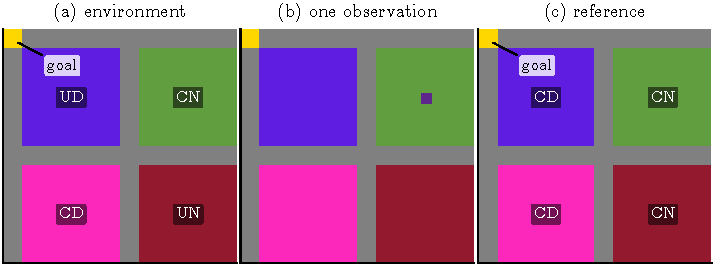
\includegraphics{fig_e3_env.pdf}
  \caption{The pixel environment of one seed (rotation of class~A). (a) Experimental environment with the dynamics
    type of each zone; (b) one observation, with the agent's marker; (c) the paired reference environment, where each
    uncontrollable zone is replaced by its controllable counterpart. The colours are the run's theme draw.}
  \label{fig:env}
\end{figure}

% =====================================================================================================================
\section{Criteria fixed in advance, and calibration}
\label{sec:criteria}
% src: notes

We tried to fix our criteria before our runs, so as not to set them to match our results.
A few were nonetheless corrected after a result (\Ks, the reading rule by zone type, the budget criterion, the tie-break
tolerance), and this is recorded as such in the log.

There are three main criteria.
% src: experiments/E3_worldmodel_4zones/aggregate_b.py (C_A, C_C, C_B_MARGIN, C_B_MIN_COUNT)
% src: docs/e3/DECISIONS.md 2026-09-23, Phase 0 validation, point 8 (the initial tolerance of C-b)
\emph{\Ca:} 99\,\% template accuracy: we decode a number of posteriors and want the nearest canonical template to be % num-ok
the right one in at least 99\,\% of cases. % num-ok
\todo{Define the templates (the pre-rendered image of each state) at their first use.}
\emph{\Cb:} the $\Lone$ error between the kernel predicted by the prior and the true kernel.
The tolerance was initially 0.1; it was then aligned with what the tabular twin measures: the criterion is computed % num-ok
only on pairs visited at least 100 times, per zone, and requires $\LoneWM \leq \LoneB + 0.05$. % num-ok
\emph{\Cc:} the linear classifier $z \to s$ must reach an accuracy of at least 99\,\%, to make sure the state % num-ok
information goes through $z$ and not through $h$.
% src: docs/e3/DECISIONS.md 2026-09-30 (4)
\Ca{} and \Cc{} are met in every run; \Cb{} is met in the deterministic zones only, not in the noisy ones (hybrid
codes, Section~\ref{sec:hybrid}).

% =====================================================================================================================
\section{The measure $\bhat$ and the tabular twin}
\label{sec:b}
% src: notes

Our measure remains $\bhat = \Ihat - \Iref$, where the reference is a real run in the paired environment, measured by
the same pipeline, so that the bias of the representation is the same on both sides and cancels.

\paragraph{Pairing rule of the reference.}
The reference environment is the same world (same grid, same permutation of the zones, same themes, same goal) in which
each uncontrollable zone is replaced by its controllable counterpart: UD becomes CD, and UN becomes CN with the same noise
level. The controllable zones do not change.
The pairing test checks that for every pair $(s, a)$, $H(s' \mid s, a)$ and the number of possible outcomes are identical
between the two worlds: only $I$ differs.
\todo[inline]{Notes vs repository: \texttt{tests/e3/test\_e3\_env.py} compares the number of outcomes for every pair $(s,a)$,
  but $H(s' \mid s, a)$ per state (\texttt{conditional\_entropy\_per\_state}), not per pair.}
In other words, the reference keeps the same level of randomness and removes only the uncontrollability; this is what
gives $\bhat = \Ihat - \Iref$ its meaning.

\paragraph{The tabular twin.}
We also have a tabular twin~\twin, which counts the same transitions as the world model but without any generalisation:
the gap between the two isolates what the representation adds.

\paragraph{Phase 0.} % num-ok
% src: docs/e3/DECISIONS.md 2026-09-23, Phase 0 validation, point 1 (the specification's 11 checkpoints)
Phase 0 (reading E2's code, not its documentation) corrected what we believed about the protocol: % num-ok
\eTwoNCheckpoints{} checkpoints and not 11, no burn-in, $\gamma = \eThreeGamma$. % num-ok

% =====================================================================================================================
\section{Agent and training loop}
\label{sec:agent}
% src: notes

\paragraph{Policy.}
We removed Dreamer's learned actor and replaced it with an $\varepsilon$-greedy policy, as in E2, to keep the same class
of policy.
$\varepsilon$ is the exploration probability of the policy: with probability $\varepsilon$ the agent plays a uniform
action, otherwise the best one according to its $Q$-values (ties broken at random).
$\varepsilon = \eThreeEpsilon$ in closed loop as in E2; $\varepsilon = \eThreeEpsilonOffline$ means a purely uniform
policy.
The $Q$-values come from a one-step lookahead from the prior: from the current latent state, \eThreeKAct{} draws per
action, and $Q$ is computed by Monte Carlo.
The critic is trained in imagination by $\lambda$-returns.

\paragraph{The loop.}
At the start of a run the agent acts in the environment to fill the replay buffer minimally (with the same policy as the
rest of the run, counted in the budget), then the algorithm starts.
When acting in the real environment there is no gradient: $h$ and $z$ are updated at every step to track where the
agent is, $h$ being reset only at the start of an episode, and the frames are added to the buffer.
In parallel, at a rate of \eThreeReplayRatio{} gradient steps per environment step, \eThreeBatchWindows{} windows of
\eThreeWindowLength{} consecutive steps are drawn from the buffer and the world model is updated on them.
The posterior states of the same batch then serve as starting points of imagined trajectories (the critic's gradient
does not flow into the world model).
These trajectories are generated with the prior over a horizon of \eThreeImagHorizon{} steps (not to be confused with
E2's \eThreeEpisodeHorizon, the truncation of real episodes).
On them, the critic is trained by $\lambda$-returns, which are its targets for $V$.
There is no actor to update: the policy is recomputed at every step from the $Q$-values.
The goal head and the critic train only from the switch on (Section~\ref{sec:startup}).
Then the cycle repeats: in short, a kind of Dyna \todo{cite: Sutton \& Barto (Dyna)}.

\paragraph{Reward and goal head.}
The reward system is trivial: \eThreeGoalReward{} on arrival at the goal (the only terminal state) and
\eThreeStepReward{} for every step that does not lead to it, which settles the question of a reward head and a
continuation head.
The model only has to learn whether a state is the goal (binary; this is not ``end of episode'', since the truncation at
\eThreeEpisodeHorizon{} steps also ends an episode without being terminal).
% src: src/helplessness/agents/worldmodel/heads.py (reward and continuation read from the goal head)
From it, the predicted reward $50\,\pgoal - (1 - \pgoal)$ and the continuation $1 - \pgoal$, which multiplies % num-ok
$\gamma V$, are deduced.
This goal head is learned on real trajectories.
It is just as well that no reward head is needed, since such a head must not influence the dynamics of the model: that
is our whole framework, in which the belief of controllability lies only in the transition beliefs, not in the rewards.
The definition of the values explains why $V = \eThreeVNoGoal = \eThreeStepReward/(1 - \gamma)$ everywhere as long as % num-ok
the goal has not been reached in imagination.
To be fully rigorous, E2 should be rerun with $V$ trained by $\lambda$-returns rather than by pure value iteration (the
``tabular Dreamer'' control, which would separate the effect of the planner from that of the representation).
This has not been done; it is deferred unless the gap with E2 turns out to be ambiguous.

\paragraph{Tie-break tolerance.}
A tolerance is used to break ties between actions from their $Q$-values.
The problem met: with a relative tolerance, when the agent knew nothing, the critic's noise became a stable preference
for an arbitrary action, whereas in E2 the tabular agent has exact ties and plays uniformly.
We therefore set an absolute tolerance, \eThreeTieTol: half the $Q$ gap between an action that brings the agent closer
to the goal and one that leaves the distance unchanged, when the goal is \eThreeEpisodeHorizon{} steps away.

% =====================================================================================================================
\section{Measuring perceived controllability}
\label{sec:measure}
% src: notes

\paragraph{From \Iz{} to \Is.}
The world model overestimates $I$ because the measure cheats: $z'$ carries a trace of the action played, through $h$.
A linear probe shows that, at fixed $(s, s')$, the action $a$ can be predicted from $z'$ with an accuracy higher than
what $(s, s')$ allow: $z'$ carries a residue of the action, so $I$ increases.
In the controllable-deterministic zone, $I$ cannot exceed $\logtwo \eThreeNActions$, so the effect is smaller there than in
another zone, and $\bhat$ does not correct this bias.
The solution is to compute $\Ihat(s)$ instead of $\Ihat(z)$, since $\Ihat(s)$ does not carry this bias
(Figure~\ref{fig:iz-is}).

% src: results/E3_worldmodel_4zones/grid12x12__4zones__pair-experimental__worldmodel-gpu_e30_bridge__seed00__20260928T154841Z/recomputed
\begin{figure}[t]
  \centering
  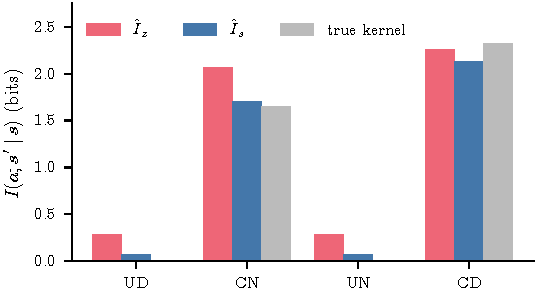
\includegraphics{fig_e3_iz_is_truth.pdf}
  \caption{Controllability by zone measured in $z$-space (\Iz) and in state space (\Is), against the true kernel's, on
    the bridge run (Section~\ref{sec:e30}; final weights, real contexts, $\Ks = \eThreeKs$ draws per pair).}
  \label{fig:iz-is}
\end{figure}

\paragraph{Real contexts.}
We initially meant to measure from a state $s$ by creating its image, then drawing from the prior with an initial \hzero{}
that carries no context and so serves as a clean baseline.
But the combination ``\hzero{} + image of an arbitrary state'' is rare during training (it only occurs at the start of a
window) and had a much lower template accuracy than real contexts; moreover, the agent does not generally act from \hzero{}
(in its trajectories it has a richer context).
We therefore moved to real contexts: the trajectories of the buffer are replayed; in each window of
\eThreeWindowLength{} steps the first \eThreeContextBurnIn{} are discarded, and for each state $s$ the frames that
correspond to it in all the remaining pieces are collected.
Up to \eThreeContextsPilot{} contexts per state (later \eThreeContextsFinal) are then drawn at random for the measures; a
state with fewer contexts gets all of them.
For $\Ihat(s)$, for instance, $\Ks = \eThreeKs$ draws are made per pair $(s, a)$, spread over the selected contexts.

\paragraph{What is measured.}
From these contexts we measure:
$\Ihat(s)$ per state and per zone (the mean of $\Ihat(s)$ over the zone), with standard errors and biases by bootstrap;
the off-support mass and \Isproj, $\Ihat(s)$ projected on the 5 reachable successors; % num-ok
% src: src/helplessness/envs/zones.py (geographic_support_mask: the 5 reachable successors)
$\Ihat(z)$ as a secondary measure;
the $\Lone$ error against $P$ and against the twin~\twin{} (criterion \Cb), the probability of the frequent outcome (T4),
the ghost rate;
\todo{Define ghosts (decoded draws matched to no template) at their first use.}
template accuracy (\Ca), the probes $z \to s$ and $h \to s$, the posterior/prior KL per zone;
\DOne{} ($\alphaapp$) and \DTwo;
the agent's $\regret$ under $P$, with its greedy policy read on the same contexts;
the prior's mass on the goal, $V$ per state and per zone, the $Q$ gaps near the goal, and the separation of the zones
in the latent.

\emph{T4} is a shape test on the noisy zones: the probability the model gives to the frequent outcome must tend to
\eThreeNoiseMain, its true value. If it stays below, the prior has not learned the right noise level. In the second GPU
batch (Section~\ref{sec:e30}) it passes in CN (\eThreeTFourCNMin{} to \eThreeTFourCNMax) but not in UN in the environment
(\eThreeTFourUNMin{} to \eThreeTFourUNMax).

\emph{\DTwo} is a diagnostic of the geometry of the latent: the Jensen-Shannon distance between the posteriors of two
neighbouring cells, comparing the pairs on either side of a boundary (zone/corridor or zone/zone) with the pairs inside
one zone. If the distances across a boundary are larger, the latent marks the zones. On the bridge run (Section~\ref{sec:e30}):
\eThreeBridgeDTwoBoundary{} bits across a boundary against \eThreeBridgeDTwoWithin{} inside a zone.

\emph{$\regret$} is the behavioural cost of the belief: $\regret(s) = \Vstar(s) - V^{\pi}(s)$, the value the agent
loses by following its greedy policy rather than the optimal one. Both values are computed exactly under the true kernel
$P$, never under the model: the policy comes from the belief, but it is judged in the true world.
$\regret \geq 0$ by construction; a negative $\regret$ signals an evaluation bug (test T9). % num-ok
It is computed for the agent (policy read on real contexts) and for the twin.

\paragraph{Limits.}
The terminal state is never a ``current state'', so it is never measured as a departure (it is measured as an arrival,
through the prior's mass on the goal); unvisited states are not measured; and the measures depend on the context.

\paragraph{Measurement noise.}
% src: docs/e3/DECISIONS.md 2026-10-06 (25) (the replays of 290,000 and 300,000 steps)
On the pilot, measured twice with the same weights at \eThreePilotBudget{} steps, $\Ihat(s)$ differed depending on whether
the buffer contained 290,000 or 300,000 frames, and this gap exceeded the standard error we had. % num-ok
This is because that standard error only measures the bootstrap uncertainty over the $K$ draws per pair, not the draw of
the contexts.
% src: docs/e3/DECISIONS.md 2026-10-07 (28) (multipliers x1, x2, x4)
We therefore tested with 1, 2 and 4 times more contexts (Figure~\ref{fig:noise}): we never quite get below the % num-ok
threshold we had set, but the noise does decrease with more contexts and costs nothing more in compute, so we keep four
times more contexts (\eThreeContextsFinal).
% src: experiments/E3_worldmodel_4zones/campaign_analysis.py (REFERENCE_EFFECT: E2's effect in the CN zone)
What was awkward is that the measurement noise with \eThreeContextsPilot{} contexts was of the same order of magnitude as
E2's bias of $-0.02$ bit in the controllable-noisy zone. % num-ok

% src: results/E3_worldmodel_4zones/gpu_pilot_noise
\begin{figure}[t]
  \centering
  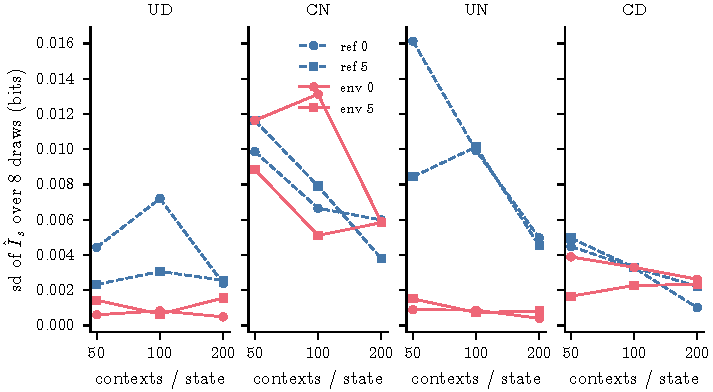
\includegraphics{fig_e3_noise.pdf}
  \caption{Measurement noise. Standard deviation of \Is{} by zone over 8 independent draws of the real contexts, % num-ok
    against the number of contexts per state. \emph{Pilot data}: final weights of the pilot's four runs (seeds
    \eThreePilotSeedA{} and \eThreePilotSeedB, environment and reference).}
  \label{fig:noise}
\end{figure}

% =====================================================================================================================
\section{Zone permutations and symmetry classes}
\label{sec:symmetry}
% src: notes

E2's code, which we reuse, permutes the zone types between the quadrants according to the seed, and an E3 test checked
whether these permutations are exact symmetries of the world.
The code rotates the zones' locations \emph{then} sets the direction of the conveyor belt, always vertical and pointing
away from the goal.
% src: docs/e3/DECISIONS.md 2026-09-23, T2 reformulated
A sketch shows that a 180-degree rotation gives the same world as the identity, but not the rotations by 90 and % num-ok
$-90$ degrees (the zone the conveyor pushes toward is no longer the same). % num-ok
This was already the case in E2, since the table is the same, but it had not been tested (E2 only checked that the
optimal values per zone type were identical).
It is of limited consequence, since from E4 on there are only two zones, but E3 should be clean: seeds are run in each % num-ok
of the two rotation classes (two per class), each run carries a class tag, and a difference between classes is
reported separately.

% =====================================================================================================================
\section{Training the world model: start-up problems}
\label{sec:startup}
% src: notes
% src: docs/e3/DECISIONS.md 2026-09-24 (entries of that day)

On 24 and 25 September we ran into successive training problems, solved one after the other, each fix revealing a % num-ok
new one.

\paragraph{The straight-through estimator.}
In DreamerV3 \todo{cite: DreamerV3}, the posterior outputs logits that form independent categorical distributions over
all latent variables (\eThreeLatentVars{} variables of \eThreeLatentClasses{} classes here); a sample of $z$ is drawn
from them, and that sample is given to the decoder.
The draw is not differentiable, so one cannot backpropagate from the decoder: the straight-through estimator sends a
sample of $z$ to the decoder but, for backpropagation, treats it as if the probabilities had been sent.

\paragraph{The first run collapsed.}
In a first run with this configuration the template accuracy was poor, the KL was identical in every zone and $\Ihat(z)$
was zero everywhere: $z$ did not encode the state, the posterior gave the same code to every state.
% src: notes (the ratio of about 1,000)
The first culprit: the code averaged the reconstruction term of the loss over all pixels, which made it about 1,000 % num-ok
times weaker than the KL term; the optimal strategy for the model was then to draw only the background and not to encode
the state in its latent, which would cost too much KL for almost no gain in reconstruction.
% src: docs/e3/DECISIONS.md 2026-09-24, posterior-collapse diagnosis (k = 2)
Moreover, the run used a reduced resolution ($k = 2$) at which the agent's marker was a single pixel; we went back to % num-ok
$k = \eThreeRenderScale$.
The reconstruction was then summed over the pixels (as in DreamerV3): necessary, but not sufficient, $z$ stayed empty.

\paragraph{Isolation test.}
% src: configs/zones/e1_4zones.yaml (144 = 12 x 12 images)
We then made an isolation test: encoder $\to z \to$ decoder alone, on the 144 images, without KL or prior. % num-ok
The same collapse occurred, so it was not due to the KL; the same test sending the probabilities to the decoder
instead of a sample worked perfectly.
The problem is the sample of $z$ sent to the decoder, and not a bug: the straight-through implementation was checked
against the analytic gradient.

Our intuition of the mechanism (the log describes the phenomenon without fully explaining it): at the start, the
posterior distributions are almost identical between states, so the samples of $z$ are only noise.
The decoder learns very quickly to reconstruct the background of the grid (the same for every state), but it also learns
to ignore $z$, which is only noise to it.
The posterior then slides towards a single, very confident code shared by every state (it does not collapse ``onto the
prior'': there is none in this test), and once it is saturated the straight-through gradient vanishes: a start-up trap.
When the samples are removed and the probabilities are sent to the decoder, the model separates the states well: even if
the differences between the states' distributions are small, the decoder can put large weights on them to amplify these
micro-differences and tell the states apart. That the decoder tells the states apart in turn lets the encoder make the
distributions more and more different between states.

\paragraph{Three estimators.}
% src: docs/e3/DECISIONS.md 2026-09-24, Categorical-bottleneck fix, point 2 (criterion: 95 % on 3 seeds)
We compared three options with a criterion fixed beforehand (at least 95\,\% on 3 seeds): straight-through alone, % num-ok
Gumbel-softmax, or probabilities first and straight-through afterwards; only the last passes (Figure~\ref{fig:estimators}).
In practice, once the states are separated, switching to straight-through does not make the model collapse again; it
even sharpens the codes.
The risk is to switch too early, before separation exists, and the moment of separation varies with the seed.

% src: results/E3_worldmodel_4zones/estimator_comparison
\begin{figure}[t]
  \centering
  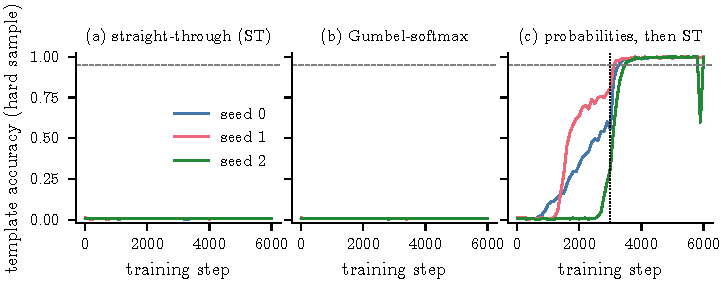
\includegraphics{fig_e3_estimators.pdf}
  \caption{Isolation test (encoder, latent, decoder; no KL), three estimators of the posterior: hard-sample template
    accuracy against the training step, three seeds each. The dashed line is the criterion fixed before the runs; the
    dotted line in (c) is the switch from probabilities to straight-through samples.}
  \label{fig:estimators}
\end{figure}

\paragraph{The switch criterion.}
At the switch the encoder must be confident enough to produce sampled codes that are distinct enough between states.
The criterion: every \eThreeSwitchEvalEvery{} steps, the Jensen-Shannon divergence between the posteriors of
\eThreeSwitchPairs{} random pairs of images of the batch is measured (without state labels, to respect the boundary
between agent and instrument), and its mean is compared with \eThreeSwitchJS{} bits (out of a possible
\eThreeLatentVars).
If it exceeds this on \eThreeSwitchConsecutive{} consecutive evaluations, the codes produced are considered distinct
enough and the switch is made; if this does not happen before a fixed deadline, the run stops with an error.
On the KL side, the term that only trains the prior ($\betadyn$) is active from the start, since it cannot cause a
collapse; the one that pulls the posterior towards the prior ($\betarep$) is at 0 until the switch and then rises % num-ok
progressively, so as not to add a counter-productive force.

\paragraph{The learning rate.}
With the specification's learning rate (\eThreeLrAfterSwitch), the states do not separate in the posterior although the
reconstruction decreases: the state is carried by micro-differences between almost uniform probabilities, which the
decoder can read, and nothing pushes the posterior to commit to a code (with the probabilities the decoder finds the
state, with a sample it does not).
Two aids failed: an entropy penalty (the posterior commits but does not separate) and progressive sampling (collapse).
With a learning rate of \eThreeLr{} the separation happens on the 3 seeds and the switch fires; we keep this learning % num-ok
rate.

\paragraph{A late collapse.}
% src: docs/e3/DECISIONS.md 2026-09-24, (i) validated; the late collapse (step 9,982; gradient about 100 times larger)
On one run (found by accident, through a measurement bug that shifted the random stream) the model collapsed in a single
step, around step 9,982, well after the switch, although it had separated the states perfectly. % num-ok
Analysing this case: after the switch the posterior is saturated, so the encoder receives tiny gradients, so its Adam
second moment is tiny; suddenly a gradient about 100 times larger than the recent ones arrives, Adam changes all the % num-ok
weights strongly and throws the posterior into a single saturated code from which it cannot come back.
The first remedy considered was gradient clipping: useless, because what matters is not the norm of the gradient (it was
ordinary) but how large it is compared with what the encoder received over the previous steps; and harmful, because
clipping broke the probabilities phase (the very large gradients at the very start are precisely what makes the
posterior depend on the image).
We therefore decided not to clip and to use a learning rate of \eThreeLrAfterSwitch{} after the switch: on the run that
collapsed, replayed identically up to the switch, this removes the collapse.
% src: docs/e3/DECISIONS.md 2026-09-25, global clipping disabled (1 event in 6 runs)
Limit: the event was seen once in 6 runs, so 6 clean runs do not prove it is gone. % num-ok
We therefore also added a guard on the JS falling back below \eThreeCollapseJS{} bit after the switch.
All our guards are meant to make a stopped run logged, not silenced and relaunched.

\paragraph{Sensitivity to the themes.}
We also looked at the model's sensitivity to the themes chosen for the zones (Figure~\ref{fig:themes}).
The switch step varies a lot from one colour draw to another (from \eThreeThemeSwitchMin{} to \eThreeThemeSwitchMax{}
steps), but several runs with the same colours vary as much, so the variation cannot be attributed to the themes: it is
mostly the randomness of training.
And \eThreeThemeCensored{} run out of \eThreeThemeRuns{} did not separate within the deadline: the start-up procedure is
not fully robust.
The optimal condition on themes will be a question to settle in E5, where it will really be critical; for now we do not
investigate further.
The switch step is now a covariate logged for every run (all the more important in E4/E5, where the colours are
manipulated); a run that does not separate is a reported failure.
One consequence of the switch is that any measure that goes through the decoder is unreadable before the switch, and
that the critic and the goal head are trained only after it.

% src: results/E3_worldmodel_4zones/theme_sensitivity
\begin{figure}[t]
  \centering
  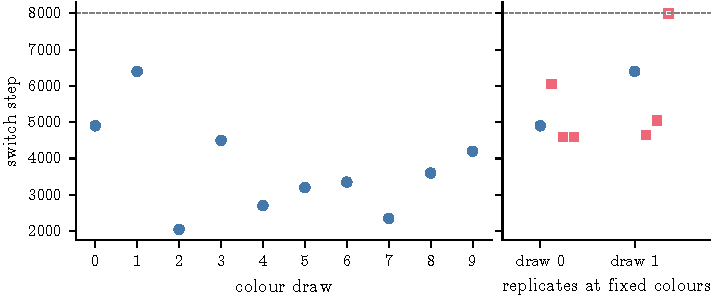
\includegraphics{fig_e3_switch_themes.pdf}
  \caption{Switch step of the probabilities phase in the isolation test. Left: ten colour draws. Right: two draws with
    three replicates each (same colours, other latent draws and minibatches); an open marker at the dashed line is a
    run that did not separate before the deadline.}
  \label{fig:themes}
\end{figure}

% =====================================================================================================================
\section{Protocol deviations found on 25 September} % num-ok
\label{sec:deviations}
% src: notes
% src: docs/e3/DECISIONS.md 2026-09-25 (episode starts; independent random streams)

A problem identified next (25 September) invalidated all the values determined before (but not the qualitative % num-ok
observations on separation).

\emph{Episode starts.} Every episode started from the terminal state, whereas in E2 the starts are uniform over the
non-terminal states. This was not a choice: the reset was called without a start state and fell back to the default cell
$(0, 0)$, which is the goal. % num-ok
It creates a heterogeneous visitation concentrated around the goal, with shorter episodes than with uniform starts (21 % num-ok
steps on average against 35.5). % num-ok

\emph{Correlated random streams.} The choice of actions, the noise of the environment and the draw of the themes each had
their own generator, but all were initialised with the same integer, so they produced exactly the same sequence of
numbers.
Streams meant to be independent were not, which seriously affects our measures, in the noisy zones especially: the draw
of the action is correlated with the triggering of the noise, while $I$ measures precisely the dependence between action
and outcome.
The specification warns that seeds correlated between an experimental run and its control were a real bug in E1; the
deviation found here is of the same kind (generators that should be independent, seeded with the same integer), within a
run.
Likewise, the measurement frequency influenced the randomness: a measurement consumed numbers from the global generator,
which shifted the latent draws of training, so measuring more or less often changed the model's learning trajectory.
We re-derived everything cleanly, as in E2 (one independent stream per use, and a separate stream per measurement),
with tests: independence of the streams, training bit-identical whatever the measurement frequency, uniformity of the
starts.

These deviations were found by a conformance test that reads the values directly in E2's code instead of copying them.
A useful consequence: seed $k$ of E3 now has the same world, the same starts and the same noise as seed $k$ of E2.
Minor problems were also fixed: incomplete metadata (permutation, themes, class A/B), episode parameters written in the
code, and the number of Monte Carlo draws for $H(z' \mid s)$, which was \eThreeIzMcTraining{} instead of the
specification's \eThreeIzMcFinal{} (decision: \eThreeIzMcTraining{} during training, \eThreeIzMcFinal{} for the final
measures).

\paragraph{\Ks.}
% src: docs/e3/DECISIONS.md 2026-09-29 (3) (K = 32 before the correction; the 0.02 floor)
Next, criterion \Cb{} could structurally not be met in the noisy zones with $K = 32$ draws as set before, because of a % num-ok
floor of estimation noise: even a perfect model, measured with 32 draws, has a mean $\Lone$ of \eThreeFloorOldK, above the % num-ok
threshold.
We kept the threshold and corrected the precision of the measure: the smallest $K$ for which this floor is at most
0.02, hence $K = \eThreeKs$. % num-ok
This correction was made after seeing the failure (it is recorded as such) but is justified independently of the model;
in any case \Cb{} still fails in the noisy zones afterwards.

% =====================================================================================================================
\section{Hybrid codes and the interpretability rule}
\label{sec:hybrid}
% src: notes

\paragraph{\Is{} is overestimated in the controllable-noisy zone.}
Where $\Ihat(z)$ was overestimated because $z'$ encoded some of the action played, $\Ihat(s)$ is overestimated too, this
time because of hybrid codes.
$\Ihat(s)$ was overestimated in the controllable-noisy zone (\eThreeZeroIsCNMin{} to \eThreeZeroIsCNMax{} against
\eThreeTrueICN{} in the second GPU batch, Section~\ref{sec:e30}), and we found that the prior assigned a non-zero mass outside
the support.
What happens is that a sample can produce a hybrid code, decoded into a real state unrelated to the support.
Part of the noise mass, which should fall on cells common to the 5 actions, then falls on cells that depend on the % num-ok
action played (this is what the rise of $H(s' \mid s)$ implies; it was not checked cell by cell), so the distributions
differ more between actions than in reality, and $\Ihat(s)$ is overestimated.

\paragraph{Two possible reasons.}
\emph{Reason A}: the prior knows the right successors, but its variables are drawn independently; for instance variable
1 can be that of outcome $\alpha$ and variable 2 that of outcome $\beta$: a hybrid code that corresponds to no real % num-ok
state and happens to be close to another state, unrelated to those of the support.
\emph{Reason B}: the prior simply believes that probable outcomes lie outside the real support, typically that it can jump
two cells.
If it is B, the prior is not trained enough and training more suffices; if it is A, it is a structural problem of the
factorised prior.
% src: docs/e3/DECISIONS.md 2026-09-30 (6) (3.6 to 5.4 times; 63 to 85 %; 26 to 37 %)
We assumed mostly A, and this was confirmed in two ways: the off-support mass is 3.6 to 5.4 times lower when each % num-ok
variable takes its most probable class (no mixing possible) than when $z$ is sampled; and most of the samples decoded off
the support are codes the posterior never produced (63 to 85\,\%, against 26 to 37\,\% of the samples in general). % num-ok
Some B remains, but A dominates.

\paragraph{A latent of 4 $\times$ 32.} % num-ok
% src: docs/e3/DECISIONS.md 2026-09-30 (6) and (7) (the 4 x 32 start-up test)
We tried a latent of 4 variables of 32 classes (fewer variables that can mix). The start-up test failed its criterion % num-ok
on 3 seeds out of 3: seeds 0 and 1 did not separate, and seed 2 separated only partly (its pair JS rose to 2.8 bits, % num-ok
below the threshold of 3 bits, a threshold that does not scale with the number of variables); with the same protocol, % num-ok
the 8 $\times$ 8 latent switched on 2 seeds out of 3. % num-ok
So we stay in \eThreeLatentVars$\times$\eThreeLatentClasses{} with this bias; the pilot later showed that longer
training reduces it clearly without removing it.

\paragraph{\Is{} and its projected version.}
We keep the measure $\Ihat(s)$ on the kernel as it is, reporting the off-support mass per zone every time, and we also
compute \Isproj, that is $\Ihat(s)$ allowing the matching only to the 5 reachable successors. % num-ok
It cannot be our main measure: we would use the environment's real dynamics to measure a belief, and would erase errors
of the model that nonetheless guide the agent; in short, we would cheat.

\paragraph{The interpretability rule.}
Our hope is that $\bhat = \Ihat - \Iref$ cancels this bias, which requires the bias to be the same on both sides.
We therefore consider $\bhat$ interpretable in a zone if $\bhat$ and $\bhat_{\mathrm{proj}}$ agree (removing the
off-support mass does not change $\bhat$, so it did not weigh in it) and if the off-support mass is the same in the
environment and in its reference.
These conditions apply only to the controllable zones, which have the same local dynamics as in their reference, so
similar off-support masses are expected.
This is not the case for an uncontrollable zone against its controllable reference (there $\bhat$ is about $-2$ bits, % num-ok
and a mass difference of 0.05 cannot explain it). % num-ok
% src: docs/e3/DECISIONS.md 2026-09-30 (7) (b about -2.2 bits; an off-support difference of 0.05)
The uncontrollable zones are not subject to this rule, but an aberration control is still made: their off-support mass
must stay within the ranges observed in \EThreeZero{}; a value outside has to be explained, not excluded.

\EThreeZero{} is the calibration condition without the loop: the data are collected at $\varepsilon =
\eThreeEpsilonOffline$, so without an agent, a goal head or a critic, and the world model is trained on them, in the
environment and in its reference. It is what ran in the first two GPU batches.

% src: docs/e3/DECISIONS.md 2026-09-30 (7), (9) and 2026-10-02 (15) (the two versions abandoned, on 2 seeds)
% src: experiments/E3_worldmodel_4zones/campaign_analysis.py (N_SEEDS, FRACTION, REFERENCE_EFFECT)
For the threshold, after two abandoned versions (computed on 2 seeds, too fragile), we anchored it on the effect we % num-ok
want to be able to detect: the effect in the controllable-noisy zone in E2 was $-0.02$ bit, so we require that, over % num-ok
the 4 seeds, the 95\,\% confidence interval of $\bhat - \bhat_{\mathrm{proj}}$ (in bits) and that of the difference % num-ok
of off-support mass (a difference of masses, without unit) both lie within $\pm 0.01$, half of this effect. % num-ok
This rule compares two versions of $\bhat$; it says nothing about the variability of $\bhat$ itself between seeds.

% =====================================================================================================================
\section{GPU runs: \EThreeZero}
\label{sec:e30}
% src: notes

\paragraph{Infrastructure.}
We then moved to GPU runs, launched by my supervisor, hence without any possible intervention during a run.
For each batch, a preflight measures the throughput before the main run and says whether to launch or stop.
The model weights at every checkpoint and the replay are stored, so that everything can be recomputed without re-running,
and for each batch a guide, \texttt{RUN\_GPU.md}, is updated for whoever launches it, with the rule that a failed run is
never relaunched without it being recorded.

\paragraph{First batch.}
The first batch was \EThreeZero{} ($\varepsilon = \eThreeEpsilonOffline$, no agent) on two seeds, as usual seed
\eThreeZeroSeedA{} (class A) and seed \eThreeZeroSeedB{} (class B), with environment and reference, \eThreeZeroEnvSteps{}
environment steps and \eThreeZeroGradSteps{} gradient steps.
The networks are the specification's (large).
A bridge run was added: the small network that had separated well on CPU, this time on GPU, with exactly the same data as
seed \eThreeZeroSeedA{} environment, to know whether a possible problem comes from the network.
% src: docs/e3/DECISIONS.md 2026-09-29 (1) (outcomes of the five runs)
Outcome: of the five runs, one completed (seed 0, reference). Two large models did not separate. One large model (seed % num-ok
5, environment) ran out of GPU memory at its first measurement (the preflight had tested the throughput only, not the % num-ok
memory of simultaneous measurements). The bridge finished its training, then ran out of GPU memory in its final
measurements, which were recomputed afterwards on CPU.

On the large models that fail, the JS starts rising and then falls back, and the posterior ends flat, at maximal entropy
(not the single code of Section~\ref{sec:startup}), while the reconstruction keeps decreasing: the state information
reaches the decoder through $h$, not through $z$.
Hence a hypothesis: with long windows, $h$ has time to carry the state, and $z$ no longer needs to separate.

\paragraph{Second batch: the shape of the windows.}
To test it, a second batch was launched with the small network (the only one that had separated), with as many images
per gradient step as the large models (\eThreeFramesPerUpdate), but with two shapes of windows:
\eThreeBatchWindows$\times$\eThreeWindowLength{} or \eThreeShortBatchWindows$\times$\eThreeShortWindowLength, same
seeds, 8 runs. % num-ok
Short windows should prevent $h$ from carrying too much information on the state, which would force $z$ to carry it.
All runs separate, and the linear probes $h \to s$ and $z \to s$ reach accuracies of \eThreeZeroProbeHMin{} to
\eThreeZeroProbeHMax{} and \eThreeZeroProbeZMin{} to \eThreeZeroProbeZMax{} respectively, in both shapes.
With the small network, the length of the windows explains nothing.
What is established is that the failures go with the large network (two runs that failed separate once the network is
changed, with identical data), but we do not know why, and we do not dig further: we keep the small network.
It is therefore not the capacity sweep planned by the specification, just a configuration that works.
We kept windows of \eThreeWindowLength{} steps, heavier for training, because the runs switch earlier (4 pairs out of 4), % num-ok
it is the specification's shape, and the final measures cost half as much; the choice was made without looking at
$\bhat$.

This batch asked two other questions, written before the launch.
Do more images per step make the kernel of the noisy zones converge? No: \Cb{} fails there in all 8 runs, which started % num-ok
the investigation of hybrid codes (Section~\ref{sec:hybrid}).
And a first floor of $\bhat$ (Figure~\ref{fig:floor}): conveyor \eThreeZeroFloorUDMax{} to \eThreeZeroFloorUDMin{}
for \eThreeTrueBUD{} in theory, controllable zones between \eThreeZeroFloorCtrlMin{} and \eThreeZeroFloorCtrlMax{} for 0, % num-ok
the uncontrollable-noisy zone not reliable.

% src: results/E3_worldmodel_4zones (the 8 gpu_e30b run directories; paper/figures/fig_e3_e30_floor.py)
\begin{figure}[t]
  \centering
  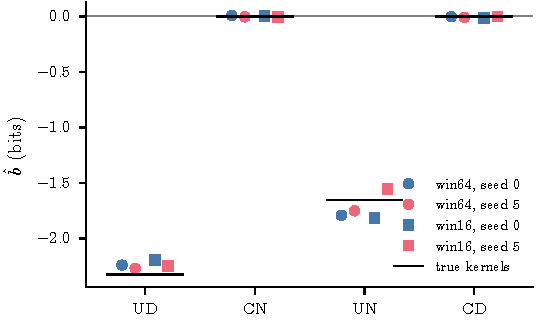
\includegraphics{fig_e3_e30_floor.pdf}
  \caption{First floor of $\bhat$ on \Is{} by zone, second GPU batch of \EThreeZero{} (two window shapes $\times$ two
    seeds, final weights), against the difference of the true kernels' controllability.}
  \label{fig:floor}
\end{figure}

\paragraph{A new role for \EThreeZero.}
Finally, the role of \EThreeZero{} was changed: it served to understand the measurement biases and to find a
configuration that learns, but the floor and the reference will come from the closed-loop campaign itself, and its values
now serve only as an aberration control (all the more since the goal's image was never stored in \EThreeZero).

% =====================================================================================================================
\section{Closed loop}
\label{sec:closed}
% src: notes

Moving to the closed loop meant fighting bugs and misunderstandings that took a lot of time.

\paragraph{Adapting choices of \EThreeZero.}
First, some choices of \EThreeZero{} had to be adapted to the closed loop.
In \EThreeZero, an entry of the buffer was the image of the current state, the action played and the reward obtained by
playing it. This convention comes from the tabular setting; as a consequence, only states from which an action is played
are stored, so the buffer never sees the terminal state.
This is not a problem under a uniform policy, but in closed loop the goal head needs to see images of the final state to
recognise it and give it $\pgoal = 1$. % num-ok
Moreover, the prior is trained to match the posterior of the next state, so images of the goal are needed in the buffer
for the prior to be able to imagine the goal state (this was not needed in \EThreeZero, since only corridor cells touch
the goal and only the zones were measured, but the gap was real).
The solution is simple: each observation is stored with the reward received on arriving at it, and at the end of every
episode that reaches the goal the goal's image is added.

Next, the goal head and the critic do not train before the switch, because before it the samples of $z$ are only noise,
so the goal head and the critic (trained on trajectories imagined by the prior, with noisy samples) would learn nothing
relevant.
% src: docs/e3/DECISIONS.md 2026-09-30 (5) F (a 90 %-greedy policy)
Previously, the output layers of these two heads were initialised at random, and the policy then followed, 90\,\% of % num-ok
the time, the arbitrary preferences of heads that had learned nothing.
They are therefore initialised at zero: all the $Q$-values are equal, and the policy is exactly uniform before the
switch, which is cleaner.
% src: docs/e3/DECISIONS.md 2026-09-30 (7) (the uniform policy's exact success rates)
Expected shapes were also fixed before reading, among them the success rate of a uniform policy, computed exactly
(0.046 in the environment, 0.117 in the reference). % num-ok

\paragraph{The mini run on CPU.}
After a first mini run on CPU, the model separates but the behaviour does not improve.
The goal head turned out to be innocent: it predicted perfectly whether a state was the goal; it was our tracking
indicator that was misleading, computed on a single batch, whereas \eThreeMiniNoGoalAtSwitch\,\% of the training batches
at the switch, and \eThreeMiniNoGoalAtResume\,\% at 18,000 steps, contained no image of the goal. % num-ok
% src: reports/diagnostics_grid12x12__4zones__pair-experimental__worldmodel-agent-agent_mini__seed00__20260930T193212Z/diagnostics.json (18,000 steps: the resume point)
The problem was the prior, which, for the pairs $(s, a)$ that lead to the goal, put a tiny mass on the goal.
So the prior never imagines reaching the goal, the reward is never obtained in imagination, and the critic learns
$V = \eThreeVNoGoal$ everywhere, the value of trajectories that wander without ever arriving.
The differences between the $Q$-values of one state are then due only to the critic's noise; this is also why the
relative tolerance was replaced by an absolute one.

We then looked for why the prior does not imagine the goal, each time with a reading rule written before the
computation (Figure~\ref{fig:mass}).

\emph{First question: a problem specific to the goal, or a general one?}
Unlike the tabular case, where one visit of a deterministic pair is enough to get the right transition, the world model
needs more visits.
% src: docs/e3/DECISIONS.md 2026-10-01 (12) a (median of the per-visit-count medians, weights at 18,000 / 20,000 steps)
The prior's median mass on the right successor of the deterministic pairs off the goal, by visits of the pair (weights at
18,000 / 20,000 environment steps), is 0.11 / 0.12 for 0--1 visits, 0.30 / 0.32 for 2--8, 0.81 / 0.79 for 9--20, % num-ok
0.94 / 0.93 for 21--50, 0.97 / 0.97 for 51--100 and 0.99 / 0.99 above 100. % num-ok
It is therefore a general insufficiency on rarely visited pairs (and not a bug: the code was reviewed).
However, among the pairs visited as often, the pairs that lead to the goal are the last of their class: the goal
receives an additional penalty, which remained to be explained.

\emph{Second question: lack of data, or under-training?}
The replay of the trained model was frozen and \eThreeMiniExtraGradSteps{} gradient steps were added, to see the mass
given to the right successor for rarely visited pairs.
It rises from \eThreeMiniMassStart{} to \eThreeMiniMassEnd: a mixed verdict, the extra gradient helps without settling
everything, and the pairs that lead to the goal keep a negligible mass.

\emph{Third question.}
At equal number of visits, a pair learns well if its arrival state has been seen often (the rule fixed in advance gives
``undetermined''; the descriptive table shows it), and the goal had been seen only \eThreeMiniGoalFrames{} times in the
buffer.
Hence the hypothesis that the goal is limited by data, and it is a circle: the goal must be reached to learn to reach it.
The only way out is a longer run.

% src: reports/diagnostics_wm_goal_grid12x12__4zones__pair-experimental__worldmodel-agent-agent_mini__seed00__20260930T193212Z
% src: reports/gradients_vs_data_grid12x12__4zones__pair-experimental__worldmodel-agent-agent_mini__seed00__20260930T193212Z
\begin{figure}[t]
  \centering
  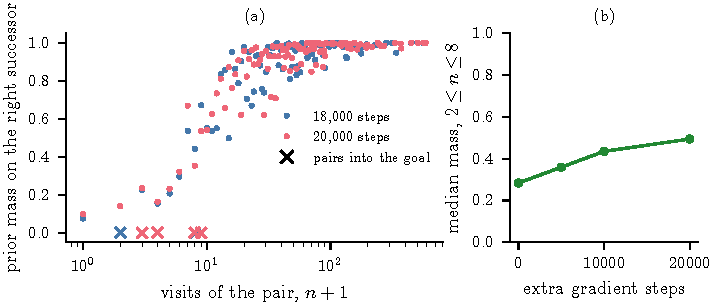
\includegraphics{fig_e3_mass_vs_visits.pdf}
  \caption{The mini run (one seed, environment). (a) Median prior mass on the right successor of the deterministic
    pairs off the goal, against the pair's visits, at two weight sets; crosses: the pairs that lead into the goal (mass
    on the goal). (b) The same median over the pairs visited 2 to 8 times after extra gradient steps on the frozen % num-ok
    replay.}
  \label{fig:mass}
\end{figure}

\paragraph{The pilot.}
We therefore launched a pilot (seeds \eThreePilotSeedA{} and \eThreePilotSeedB, environment and reference) of
\eThreePilotBudget{} steps, with windows of \eThreeBatchWindows$\times$\eThreeWindowLength{} and a ratio of
\eThreeReplayRatio{} gradient steps per environment step instead of \eThreeReplayRatioMini, since the goal problem is a
problem of data, not of gradient (and with this larger batch it still makes more replayed images per step than in the
mini run).
Result (Figure~\ref{fig:pilot}): it works; the four runs end with a mass of \eThreePilotGoalMassFinal{} on the goal and
a success close to 100\,\%, and the hypothesis is confirmed. % num-ok
% src: docs/e3/DECISIONS.md 2026-10-06 (27) (about 19 to 36 for the uniform policy)
The agent's $\regret$ falls to between \eThreePilotDeltaMin{} and \eThreePilotDeltaMax{} by zone, against 19 to 36 for % num-ok
a uniform policy.

% src: results/E3_worldmodel_4zones (the four pilot run directories, gpu_pilot_closed_loop; paper/figures/fig_e3_pilot_learning.py)
\begin{figure}[t]
  \centering
  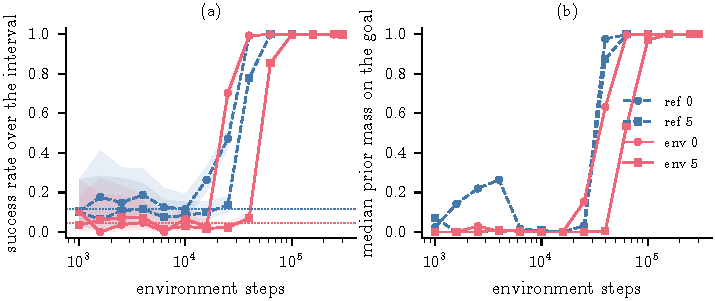
\includegraphics{fig_e3_pilot_learning.pdf}
  \caption{The closed-loop pilot. \emph{Pilot data}: seeds \eThreePilotSeedA{} and \eThreePilotSeedB, environment
    (env) and reference (ref). (a) Success rate over each interval between two checkpoints, with its 95\,\% Wilson % num-ok
    interval; dotted lines: the uniform policy's exact rate in each world. (b) Median prior mass on the goal over the
    four pairs that lead into it.}
  \label{fig:pilot}
\end{figure}

\paragraph{Intervals still unexplained.}
Once this problem was solved, a question remained: in two intervals, the success was well above chance without the prior
putting mass on the goal, so where does the information go through?
A first diagnostic concluded to a ``generalisation of $V$'', a wrong label: reading the code again, the critic is trained
only in imagination; it can know nothing of the goal if the prior never imagines it.
% src: docs/e3/DECISIONS.md 2026-10-07 (28), task b (masses 0 to 0.0008; one pair at 0 of 10,000)
With more draws (\eThreeGoalDraws{} instead of \eThreeGoalDrawsPilot), the masses on the goal are all below $1/256$: % num-ok
three of the four pairs have a non-zero mass (at most 0.0008), the fourth has exactly 0 of \eThreeGoalDraws; but the % num-ok
$Q$ gaps stay below the tolerance, so there is no explanation to date.
It concerns only two intervals, early in the run, and the values of $V$ and $Q$ near the goal are logged at every
checkpoint of the campaign, so we can come back to it.

\paragraph{The budget.}
Finally, the campaign's budget had to be fixed by a criterion.
The first criterion, $\Ihat(s)$ stable between two checkpoints, had a threshold smaller than the measurement noise, hence
unattainable by construction (this is how we discovered this noise and fixed the protocol with four times more
contexts).
The corrected criterion: the agent must have finished learning, and $\Ihat(s)$ must vary by less than two standard
deviations of the measurement noise.
No checkpoint satisfies it, so the budget stays at \eThreeBudget{} by default: it is not a convergence point,
$\Ihat(s)$ still rises in the controllable-noisy zone and in the noisy zones of the references (Figure~\ref{fig:pilot-is}).
To keep in mind for the analysis: once the agent knows how to reach the goal the visitation is no longer uniform (hence
the analysis of $\bhat$ by visit class), and seeds \eThreePilotSeedA{} and \eThreePilotSeedB{} of the campaign are the
pilot's runs, measured again, whose $\bhat$ we have already seen.

% src: results/E3_worldmodel_4zones/gpu_pilot_remeasure
\begin{figure}[t]
  \centering
  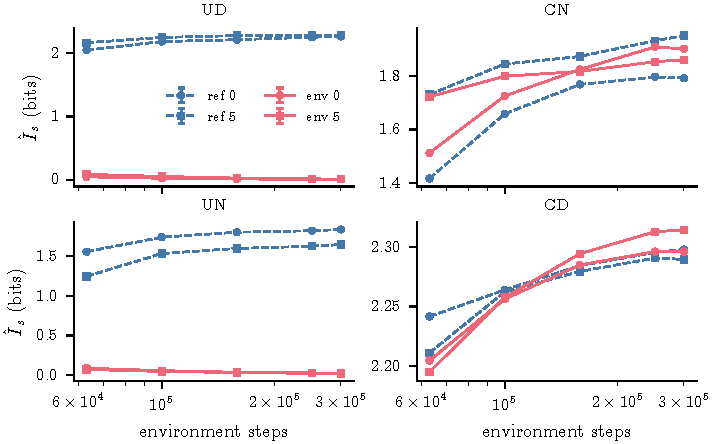
\includegraphics{fig_e3_pilot_is.pdf}
  \caption{\Is{} by zone at the re-measured checkpoints of the pilot, with its bootstrap standard error. \emph{Pilot
    data}: seeds \eThreePilotSeedA{} and \eThreePilotSeedB, environment (env) and reference (ref), measured with
    \eThreeContextsPilot{} contexts per state; the last point is measured on the replay of the last saved resume point.}
  \label{fig:pilot-is}
\end{figure}

% =====================================================================================================================
\section{The final campaign: design and analyses}
\label{sec:campaign}
% src: notes

Once all this was clarified, we moved to the final run of E3, which aims to give us the baseline, the floor and a
characterisation of all our measures in a four-zone environment without perceptual similarity.
As I write, the batch is running, so its results will come at the end; here I present what we measure, our expectations
and the limits.

\paragraph{Runs.}
Seeds \eThreeCampaignSeedA{} (class A) and \eThreeCampaignSeedB{} (class B) run on the environment and its reference,
in the same conditions as the last pilot.
Seeds \eThreePilotSeedA{} and \eThreePilotSeedB{} should also run, but since this was already done in the same
conditions, the pilot's weights saved at every checkpoint are reused and all the measures are redone on them with the
campaign's protocol (we checked that the campaign's training code is identical to the pilot's).
% src: docs/e3/DECISIONS.md 2026-10-07 (30) (replay of 290,000 steps; about 3.5 days and 2 days)
The only reservation: their last point, at \eThreeBudget{} steps, is measured on the replay at 290,000 steps, the last % num-ok
one saved. The final run thus goes from about 3.5 days to 2 days, which is not negligible. % num-ok
For transparency: these pilot runs served to fix the budget (on the stability of $\Ihat(s)$ and the agent's learning,
never on $\bhat$), and we have already seen their $\bhat$; the analyses, however, were fixed before.

\paragraph{Measures.}
% src: docs/e3/DECISIONS.md 2026-10-07 (29) (8 or 9 checkpoints after the switch)
During the runs, at every checkpoint after the switch (8 or 9 per run), the full measures are made: $\Ihat(s)$, % num-ok
\Isproj, $\Ihat(z)$, the off-support mass, the kernels, the probes.
At every checkpoint: the counts, the tabular twin, the prior's mass on the goal with \eThreeGoalDraws{} draws, the $Q$
gaps near the goal, $V$ by zone, and the separation of the zones in the latent.
The weights and the counts are saved at every checkpoint, as well as the final replay, so everything can be recomputed
afterwards, off the cluster.

\paragraph{Main analysis.}
The main metric is $\bhat$ by zone, computed from $\Ihat(s)$, at \eThreeBudget{} steps.
It comes with the rule on hybrid codes in the controllable zones and with the aberration control against the ranges of
\EThreeZero.

\paragraph{Secondary analyses.}
The following analyses are secondary, but no less important to prepare the rest of the study.

\emph{$\bhat$ by visit class.} The aim is to separate the effect of the representation from the effect of the amount of
data, since the agent does not visit the same places in the environment and in the reference.
% src: experiments/E3_worldmodel_4zones/campaign_analysis.py (VISIT_CLASSES)
The states are grouped into visit classes (0--9, 10--29, 30--99, \ldots) by the number of visits of their least-played % num-ok
action, and $\bhat$ between environment and reference is computed within each class.

\emph{The difference of differences.} $\Ihat_{\mathrm{WM}} - \Ihat_{\mathrm{twin}}$ is computed in the environment and in
the reference, and the two are subtracted.
The idea was to isolate what the representation adds at identical data; but, checked on the pilot, the twin is close to
the truth on both sides, so the difference of differences is about $\bhat$ itself and varies as much between seeds: it is
reported as descriptive.

\emph{$\alphaind$} (not to be confused with $\alphaapp$ of \DOne). For each state, the predicted kernel is fitted as a
mixture $(1 - \alphaind)\,P + \alphaind\, m$, with $P$ the true kernel and $m$ a distribution shared by every action. % num-ok
$\alphaind = 0$ means that the model believes in the right effects of its actions, $\alphaind = 1$ that it believes the % num-ok
outcome does not depend on the action; it is our estimate of the model's belief of uncontrollability in this state (not
defined in the uncontrollable zones of the environment, and not bounded between 0 and 1). % num-ok

\emph{Zones in the latent.} A linear probe predicts the zone from $(h, z)$, then whether the zone is controllable; in the
reference every zone is controllable, so there it separates appearances only and serves as a control.

\paragraph{Expectations.}
Roughly, we expect zero generalisation at the budget in the controllable zones ($\bhat \approx 0$ and % num-ok
$\alphaind \approx 0$: zones perceived as different, which the model separates well), with a possible transient effect % num-ok
early in learning.
A null result will be reported as a bound (no effect larger than our resolution), not as an absence of effect.

\paragraph{Limits known in advance.}
% src: experiments/E3_worldmodel_4zones/campaign_analysis.py (REFERENCE_EFFECT, N_SEEDS)
In the controllable-noisy zone, the spread between seeds seen on the pilot is much larger than E2's effect ($-0.02$ % num-ok
bit), so with 4 seeds an effect of this size cannot be detected. % num-ok
The rule on hybrid codes may declare a zone not interpretable, and this will be reported as it is.
\eThreeBudget{} steps is not a convergence point: $\Ihat(s)$ still rises.
And with two seeds per class, a difference between classes A and B can be described but not tested.

% =====================================================================================================================
\section{Results of the final campaign}
\label{sec:results}
% src: docs/E3_worldmodel_4zones.md (results section, between the e3-campaign-results markers)
% src: docs/e3/DECISIONS.md 2026-10-13 (31), (32); 2026-10-14 (33) to (36)
% src: docs/e3/campaign_tables/analysis.json (the campaign pipeline's output, copied from results/E3_worldmodel_4zones/campaign/)

Seeds \eThreeCampaignSeedA{} and \eThreeCampaignSeedB{} are new closed-loop runs; seeds \eThreePilotSeedA{} and
\eThreePilotSeedB{} are the pilot's runs measured again with the campaign's protocol (four times the contexts, every
measure at every checkpoint after the switch). Each seed has an environment run and a paired reference run. The budget
is \eThreeBudget{} environment steps. Every rule, threshold and expected shape was recorded in \texttt{DECISIONS.md}
before the data were read ((16), (29) to (32)); the corrections made after a result are recorded as such ((33), (35)), % num-ok
and so is the exploratory analysis of seed \eThreeCampaignSeedA{} ((34) to (36)). With $N = 4$ seeds every statement is % num-ok
descriptive. A null result is reported as a bound, the largest end of the 95\,\% Student-t interval over the seeds, % num-ok
never as the absence of an effect.
All 8 jobs finished (exit code 0, \eThreeBudget{} environment steps, complete archives, no interruption); the switches % num-ok
occurred between environment steps 8,175 and 17,008, and each run was fully measured at 7 to 9 checkpoints after its % num-ok
switch. The pilot runs' last checkpoint rests on the replay at 290,000 steps (flagged). % num-ok

% =====================================================================================================================
\subsection{The model and the agent work in closed loop}
\label{sec:results-loop}

At the budget every run reaches the goal and its goal is learnt: the success over the last interval is 0.999 to 1.000, % num-ok
the prior's median mass on the goal 0.997 to 1.000, and the $Q$ gaps next to the goal 6.6 to 15.7, far above the % num-ok
tie-break tolerance (\eThreeTieTol). \Ca{} is at least 0.996 in every run, and \Cc{} too except in seed % num-ok
\eThreeCampaignSeedA{}'s environment (0.976). % num-ok

The deterministic zones are learnt: at \eThreeBudget{} steps the prior's mass on the true successor is 0.94 to 0.99 in % num-ok
the deterministic zones, lower in the CD zone of seed \eThreeCampaignSeedA{}'s environment (0.91). The tabular twin's % num-ok
$\Lone$ error falls in every zone. \Cb{} holds in UD in every run and fails in the noisy zones in every run, as in
calibration; in CD and the corridor it fails in some runs (seed \eThreeCampaignSeedA{}'s environment in both zones, seed
\eThreeCampaignSeedB{}'s reference in the corridor).

In the uncontrollable zones, $\bhat$ is close to its theoretical value (Table~\ref{tab:campaign-b},
Figure~\ref{fig:campaign-maps}): \eThreeCampaignBUDMean{} [\eThreeCampaignBUDLow, \eThreeCampaignBUDHigh] bits in UD,
for $-\logtwo \eThreeNActions$ in theory, and \eThreeCampaignBUNMean{} [\eThreeCampaignBUNLow, \eThreeCampaignBUNHigh]
in UN, for $-$\eThreeTrueICN.

% src: docs/e3/campaign_figures/maps_300000.png
\begin{figure}[t]
  \centering
  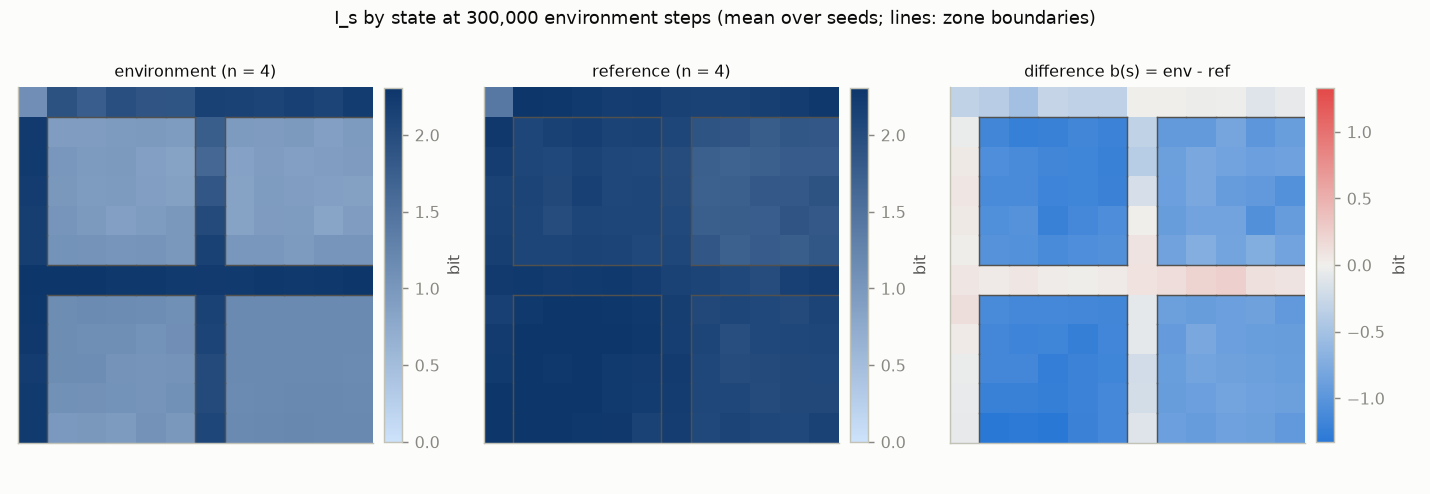
\includegraphics[width=\linewidth]{../../docs/e3/campaign_figures/maps_300000.png}
  \caption{\Is{} by state at \eThreeBudget{} environment steps, mean over the 4 seeds: environment (left), reference % num-ok
    (middle) and their difference $\bhat(s)$ (right). The maps are drawn in the grid's own coordinates and average
    seeds whose zone types occupy different quadrants (E2's counterbalancing), so a quadrant block is not a single zone
    type; the cross between the blocks is the corridor. Lines: zone boundaries.}
  \label{fig:campaign-maps}
\end{figure}

% =====================================================================================================================
\subsection{Main result: no propagation of uncontrollability beyond the resolution obtained}
\label{sec:results-main}

In the controllable zones, $\bhat$ and $\alphaind_{\mathrm{env}} - \alphaind_{\mathrm{ref}}$ are compatible with 0 at % num-ok
the budget, as expected ((29), (31); Table~\ref{tab:campaign-b}, Figure~\ref{fig:campaign-curves}). % num-ok
No effect of the uncontrollable zones on the controllable ones larger than the bounds is detected: \eThreeCampaignBoundCN{}
bit in CN, \eThreeCampaignBoundCD{} bit in CD and \eThreeCampaignBoundCorridor{} bit in the corridor. This is a bound on
an effect, about 0.2 to 0.3 bit, not the absence of an effect. % num-ok
In CN and CD this reading is subject to the hybrid-code rule, which is not satisfied (Section~\ref{sec:results-noisy}).

\begin{table}[t]
  \centering
  \small
  \begin{tabular}{lccc}
    \toprule
    zone & $\bhat$, mean [95\,\% CI] (bits) & bound of a null & $\alphaind_{\mathrm{env}} - \alphaind_{\mathrm{ref}}$ [95\,\% CI] \\ % num-ok
    \midrule
    UD & \eThreeCampaignBUDMean{} [\eThreeCampaignBUDLow, \eThreeCampaignBUDHigh] & & not defined \\
    UN & \eThreeCampaignBUNMean{} [\eThreeCampaignBUNLow, \eThreeCampaignBUNHigh] & & not defined \\
    CN & \eThreeCampaignBCNMean{} [\eThreeCampaignBCNLow, \eThreeCampaignBCNHigh] & \eThreeCampaignBoundCN
       & \eThreeCampaignDAlphaCNMean{} [\eThreeCampaignDAlphaCNLow, \eThreeCampaignDAlphaCNHigh] \\
    CD & \eThreeCampaignBCDMean{} [\eThreeCampaignBCDLow, \eThreeCampaignBCDHigh] & \eThreeCampaignBoundCD
       & \eThreeCampaignDAlphaCDMean{} [\eThreeCampaignDAlphaCDLow, \eThreeCampaignDAlphaCDHigh] \\
    corridor & \eThreeCampaignBCorridorMean{} [\eThreeCampaignBCorridorLow, \eThreeCampaignBCorridorHigh]
       & \eThreeCampaignBoundCorridor
       & \eThreeCampaignDAlphaCorridorMean{} [\eThreeCampaignDAlphaCorridorLow, \eThreeCampaignDAlphaCorridorHigh] \\
    \bottomrule
  \end{tabular}
  \caption{$\bhat = \Is(\mathrm{env}) - \Is(\mathrm{ref})$ and the difference of the action-independent weight
    $\alphaind$ by zone at \eThreeBudget{} environment steps: mean over the 4 seeds and 95\,\% Student-t interval; the % num-ok
    bound of a null is the largest end of the interval. $\alphaind$ is not defined in the uncontrollable zones of the
    environment.}
  \label{tab:campaign-b}
\end{table}

The secondary analyses of propagation, with their rules recorded before the data ((31) D, descriptive thresholds), % num-ok
point the same way:
\begin{itemize}
  \item \emph{$\bhat$ at equal visits}, with the training time as a covariate: the intercept $b_0$ is compatible with 0 % num-ok
    in CN, CD and the corridor (bounds 0.20, 0.54 and 0.38 bit); the training-time term is positive in every zone % num-ok
    (+0.75 to +1.03 per decade of the checkpoint). % num-ok
  \item \emph{$\bhat$ against the distance to the nearest uncontrollable zone} (main zone CD): the propagation shape is
    absent at every checkpoint. In the secondary zones the rule's ``present'' verdict occurs in CN at 100,000 and % num-ok
    300,000 steps and in the corridor at 100,000. % num-ok
  \item \emph{Useful generalisation} (world model against the twin on pairs visited at most 10 times; ``negative in all % num-ok
    4 seeds'' is a one-sided sign test at $p = 1/16$): the world model does not generalise better than the twin in UD, % num-ok
    UN and the corridor of the environment up to 63,096 steps; every other cell is not testable. % num-ok
\end{itemize}

% src: docs/e3/campaign_figures/curves_b_alpha.png
\begin{figure}[t]
  \centering
  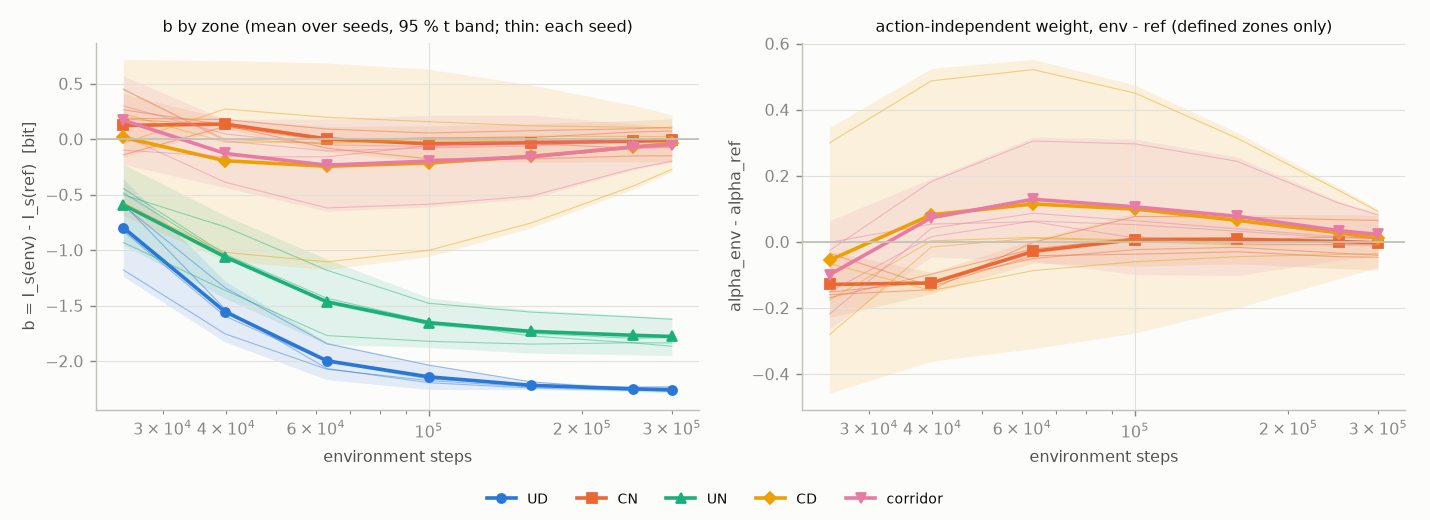
\includegraphics[width=\linewidth]{../../docs/e3/campaign_figures/curves_b_alpha.png}
  \caption{Left: $\bhat$ by zone against the environment steps, at the checkpoints measured in every pair (mean over the
    4 seeds with its 95\,\% Student-t band; thin lines: each seed). Right: $\alphaind_{\mathrm{env}} - % num-ok
    \alphaind_{\mathrm{ref}}$, the difference of the weight of an action-independent component in the predicted kernel,
    in the zones where it is defined.}
  \label{fig:campaign-curves}
\end{figure}

% =====================================================================================================================
\subsection{The early transient in CN: a visitation effect}
\label{sec:results-transient}

$\bhat$ in CN is positive at 39,811 steps (\eThreeCampaignBCNEarlyMean{} [\eThreeCampaignBCNEarlyLow, % num-ok
\eThreeCampaignBCNEarlyHigh]), and $\alphaind_{\mathrm{env}} - \alphaind_{\mathrm{ref}}$ is negative at 25,119 and 39,811 % num-ok
(Figure~\ref{fig:campaign-curves}). This goes in the direction opposite to a propagation of uncontrollability, which
would give $\bhat < 0$. At equal visits $\bhat$ in CN is about 0 ($b_0 = \eThreeCampaignBZeroCNMean$ % num-ok
[\eThreeCampaignBZeroCNLow, \eThreeCampaignBZeroCNHigh]). Early on, CN receives a larger share of the visits in the
environment than in the reference in 3 of the 4 seeds (seed \eThreeCampaignSeedA: 0.27 and 0.29 of all visits at 25,119 % num-ok
and 39,811 steps, against 0.10 and 0.11). The transient is therefore read as a visitation effect, not as a propagation. % num-ok
This reading is a correction made after the result ((34), (35)): the transient had first been reported as the % num-ok
anticipated early effect; no rule and no recorded result was modified.

% =====================================================================================================================
\subsection{Organisation of the latent (RSA)}
\label{sec:results-rsa}

At the state level, the distances between the model's latent states are explained modestly by the theoretical
matrices ($R^2$ at \eThreeBudget{} steps: 0.32 in the environment and 0.54 in the reference on $h$, 0.12 and 0.17 on % num-ok
$z$), mostly through the position on the torus (unique share 0.24 and 0.42 on $h$, 0.08 and 0.13 on $z$; % num-ok
Figure~\ref{fig:campaign-rsa}). The unique share of the controllability matrix is 0.001 to 0.005. The predictors are % num-ok
weakly collinear (variance inflation factor at most 1.8), and no regression weight is read in isolation. % num-ok
In E3, however, theme, position and zone are confounded: each theme occupies one fixed region of the torus, so E3
cannot separate theme from position.
The confusion ratio between controllable and uncontrollable zones (grouped by appearance; corrected after the first run
of the pipeline, (33)) is, on $h$, lower in the environment than in the reference from 39,811 to 251,189 steps % num-ok
(interval excluding 0), and $-0.086$ [$-0.187$, $+0.016$] at \eThreeBudget{} steps; on $z$ it is compatible with 0 at % num-ok
every checkpoint. The CD versus UD and CN versus UN ratios are compatible with 0 everywhere. % num-ok
The distance on $z$ is the sum over the \eThreeLatentVars{} categorical variables of their Jensen-Shannon divergences,
not the divergence of the joint distribution.

% src: docs/e3/campaign_tables/analysis.json (rsa_over_seeds, partition)
\begin{figure}[t]
  \centering
  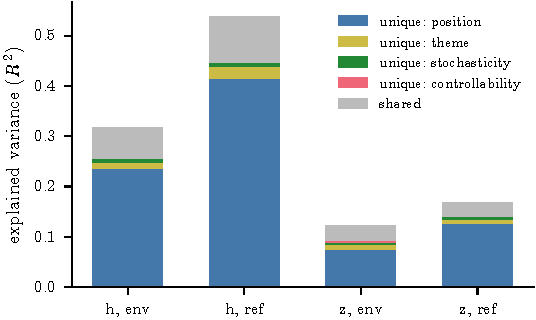
\includegraphics{fig_e3_rsa_partition.pdf}
  \caption{RSA of the latent at \eThreeBudget{} environment steps (mean over the 4 seeds): variance of the state-level % num-ok
    distances between latent states explained by the theoretical matrices, split into each predictor's unique share and
    the shared share; the bar height is $R^2$. In the reference every zone is controllable, so the controllability % num-ok
    predictor is constant and removed. Theme, position and zone are confounded in E3.}
  \label{fig:campaign-rsa}
\end{figure}

% =====================================================================================================================
\subsection{Seed \eThreeCampaignSeedA: an exploratory observation}
\label{sec:results-seed}

Seed \eThreeCampaignSeedA's environment run learns CD much more slowly than the other runs
(Figure~\ref{fig:campaign-seed}): the prior's mass on the true successor goes from 0.28 (15,849 steps) to 0.91 % num-ok
(\eThreeBudget{} steps), against at least 0.97 from 63,096 steps in seed \eThreeCampaignSeedB. $\bhat(\mathrm{CD})$ is % num-ok
$-0.27$ at \eThreeBudget{} steps, against $-0.04$ to $+0.10$ in the other seeds. This run alone makes the convergence % num-ok
criterion fail (Section~\ref{sec:results-limits}).
The following diagnostics are exploratory and post hoc ($\bhat(\mathrm{CD})$ had been seen), each with its rule
recorded before computing it.
{\sloppy
\begin{itemize}
  \item \emph{(34), ``helplessness'' against ``failed learning'' signature: undetermined.} $\alphaind$ in CD exceeds the % num-ok
    other runs and its reference (+0.091 against a threshold of 0.05), but the errors are not concentrated near the % num-ok
    boundary ($\rho(\text{error}, \text{distance}) = +0.22$) and they are concentrated on little-visited states % num-ok
    ($\rho(\text{error}, n) = -0.55$). % num-ok
  \item \emph{A design flaw of (34)'s rule, recorded after the result ((35)).} A high $\alphaind$ is the normal % num-ok
    signature of early learning in every run (an action-independent prediction before the actions' effects are
    learnt), so $\alphaind$ compared at the same checkpoint cannot distinguish a delay of learning from a belief of
    helplessness. (34)'s verdict stays recorded as it was obtained. % num-ok
  \item \emph{(35), $\alphaind$ against the visits $n(s)$.} Per state, seed \eThreeCampaignSeedA's $\alphaind$ stays % num-ok
    above the other runs' range at equal visits in 3 of 4 qualifying bins: ``effect proper to this model''; on zone % num-ok
    means the verdict is undetermined. Over its first \textasciitilde25,000 steps, this run gave the smallest share of % num-ok
    its visits to CD (0.14, against 0.20 to 0.34) and the largest to CN (0.27, against 0.10 to 0.18). % num-ok
  \item \emph{(36), the timing of the visits} ($\alphaind$ regressed on $\log_{10} n$ and on the mean step of the % num-ok
    state's visits): the timing coefficient is negative ($-0.172$ per 100,000 steps [$-0.207$, $-0.134$]), later visits % num-ok
    going with a smaller $\alphaind$, opposite to the loss-of-plasticity hypothesis; seed \eThreeCampaignSeedA's mean
    residual stays outside the other runs' range with or without the term (+0.160 without, +0.180 with, against % num-ok
    [$-0.085$, $+0.026$] and [$-0.091$, $+0.013$]). Verdict: the gap persists; it is proper to this model, with no % num-ok
    explanation identified.
\end{itemize}
\par}
The candidate explanations, as they stand after these tests: a delay of learning due to few early visits to CD
(consistent with the visit shares, but it does not account for the per-state gap at equal visits); a loss of plasticity
or primacy bias (not supported: the timing term has the opposite sign); a helplessness-like belief propagated from the
uncontrollable zones (not supported by the spatial pattern of the errors); a property of this run's training trajectory
(initialisation, optimisation) not captured by the visits or their timing (not tested).

% src: docs/e3/campaign_figures/cd_learning.png
% src: docs/e3/campaign_figures/visit_timing.png
\begin{figure}[t]
  \centering
  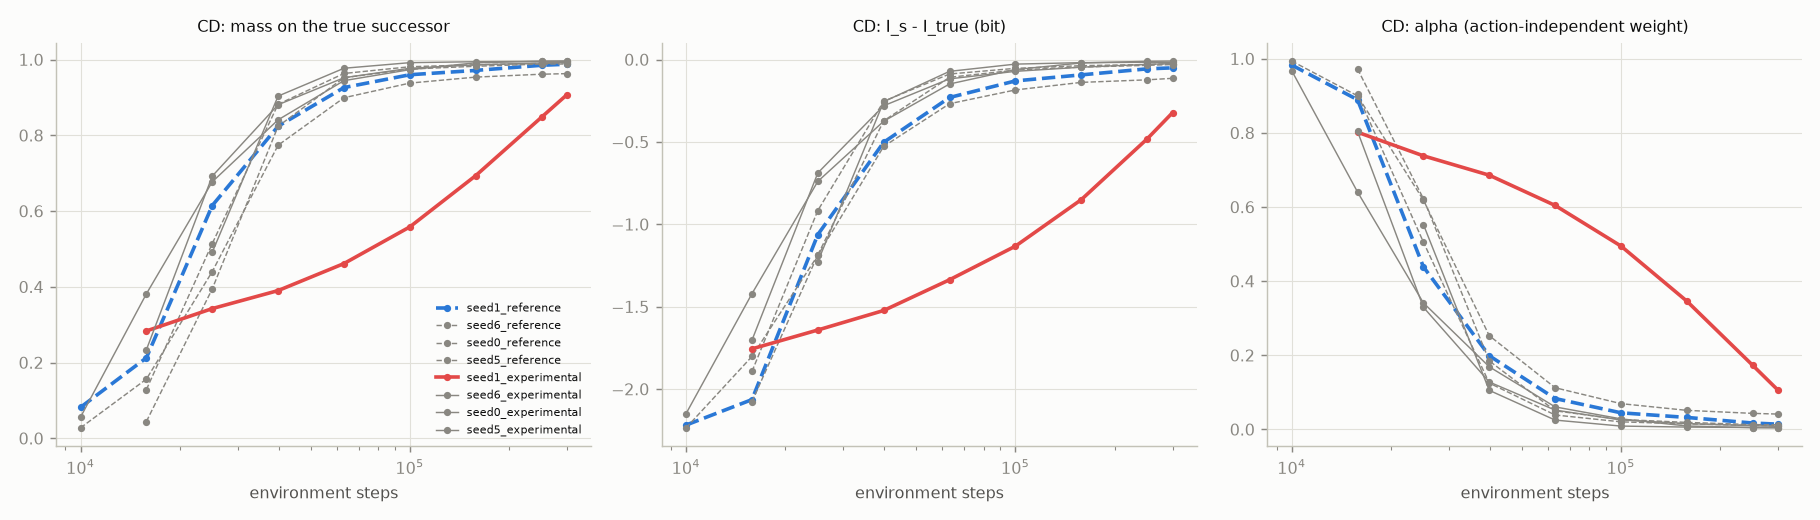
\includegraphics[width=\linewidth]{../../docs/e3/campaign_figures/cd_learning.png}\\[4pt]
  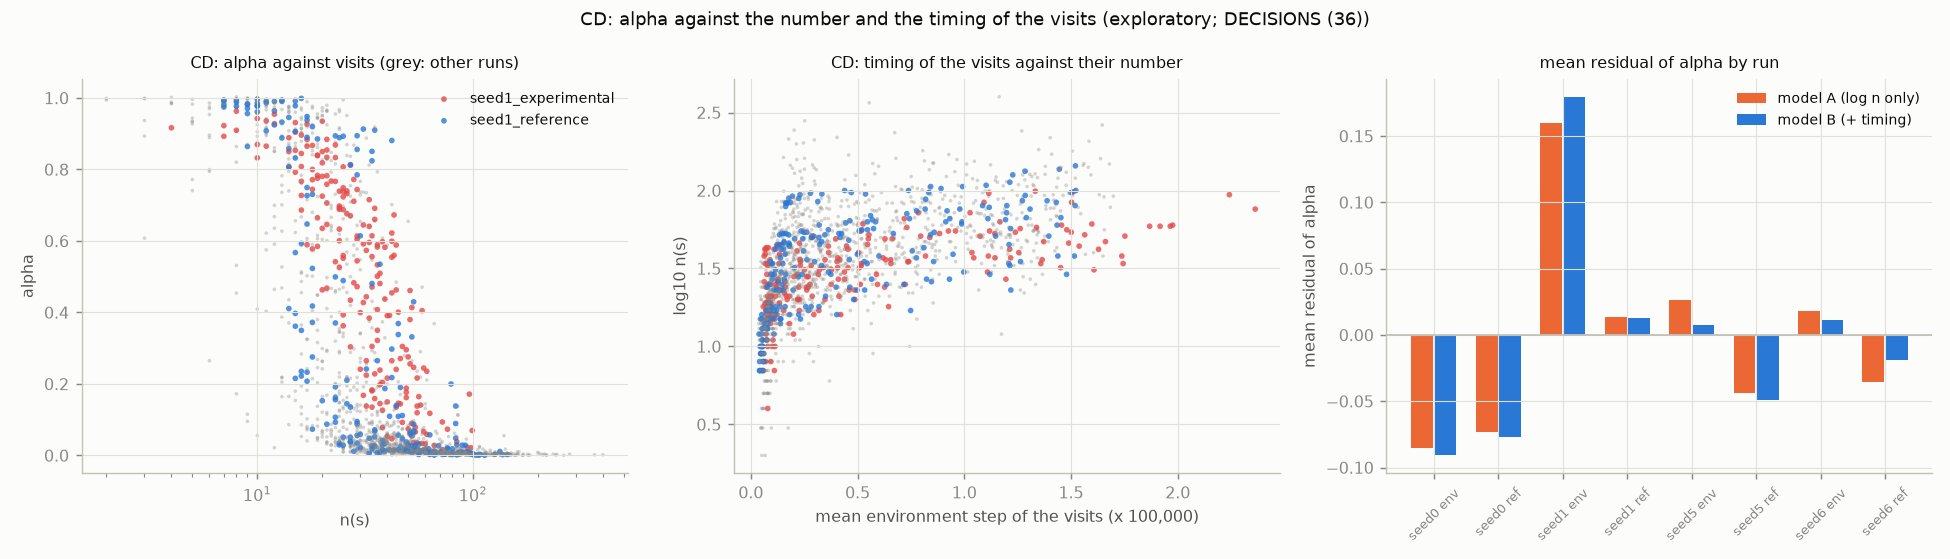
\includegraphics[width=\linewidth]{../../docs/e3/campaign_figures/visit_timing.png}
  \caption{Seed \eThreeCampaignSeedA{} (exploratory, post hoc). Top: the CD zone in every run against the environment
    steps, prior's mass on the true successor, $\Is - I_{\mathrm{true}}$ and $\alphaind$ (red: seed
    \eThreeCampaignSeedA's environment; blue dashed: its reference; grey: the other runs). Bottom ((36)): $\alphaind$ % num-ok
    per CD state against the visits, the timing of the visits against their number, and each run's mean residual of
    $\alphaind$ without (model A) and with (model B) the timing term.}
  \label{fig:campaign-seed}
\end{figure}

% =====================================================================================================================
\subsection{The noisy zones}
\label{sec:results-noisy}

\emph{Measurement error.} In CN, \Is{} exceeds the true kernel's controllability by +0.211 (sd 0.072) in the % num-ok
environment and +0.222 (0.073) in the reference at \eThreeBudget{} steps; the excess was negative early ($-0.83$ and % num-ok
$-0.95$ at 25,119 steps) and grows with training. The resolution that a four-seed extension to the noisy zones would % num-ok
have on $\bhat$ (the half-width of its 95\,\% interval) is 0.19 bit in CN and 0.17 bit in UN at \eThreeBudget{} steps. % num-ok

\emph{The hybrid-code rule (29) is not satisfied.} In CN and CD, the 95\,\% intervals of % num-ok
$\bhat(\Is) - \bhat(\Isproj)$ and of the difference of off-support mass between the environment and the reference
exceed $\pm 0.01$ (CN: $-0.0027$ [$-0.0209$, $+0.0156$] and $-0.0040$ [$-0.0249$, $+0.0170$]; CD: $-0.0082$ % num-ok
[$-0.0395$, $+0.0230$] and $+0.0026$ [$-0.0346$, $+0.0399$]). $\bhat$ is therefore not interpretable in these zones % num-ok
under the rule fixed before the campaign.

\emph{Aberration control against \EThreeZero.} Twelve values are flagged, none excluded: in all 4 seeds the % num-ok
environment's off-support mass is below \EThreeZero's intervals in UD and UN, as already in the pilot ((22)); in 3 seeds % num-ok
the difference of off-support mass between environment and reference in CD exceeds its threshold; in seed
\eThreeCampaignSeedB{}, $|\bhat(\Is) - \bhat(\Isproj)|$ in CD exceeds its threshold (0.029 against 0.0285). % num-ok

The noisy zones thus carry a measurement error of about 0.2 bit that grows with training, and the bias of the hybrid % num-ok
codes, whereas the deterministic zones are learnt with a mass of 0.94 to 0.99 on the true successor. This is why the % num-ok
next steps of the study are carried out in deterministic zones.

% =====================================================================================================================
\subsection{Limits}
\label{sec:results-limits}

\begin{itemize}
  \item \emph{$N = 4$ seeds.} Every result is descriptive. The bounds on $\bhat$ in the controllable zones, about 0.2 to % num-ok
    0.3 bit, come from the variability between seeds; they are roughly ten times E2's effect in CN % num-ok
    (\eTwoEffectCN{} bit). E3 can only exclude effects larger than these bounds.
  \item \emph{The hybrid-code rule (29) is not satisfied} in CN and CD: $\bhat$ is not interpretable there under the % num-ok
    rule fixed before the campaign.
  \item \emph{The budget was not reduced.} No candidate checkpoint satisfies the convergence criterion of the
    deterministic zones ((31) E), so the budget of the next runs stays at \eThreeBudget{} steps: the agent-learning % num-ok
    condition fails at every candidate because of seed \eThreeCampaignSeedA's environment, and the stability of \Is{} in
    UD, CD and the corridor (Bonferroni-corrected thresholds, 0.007 to 0.011 bit) fails up to the last step, mostly in % num-ok
    that run.
  \item \emph{A design flaw of (34)'s rule}, recorded after the result ((35)): $\alphaind$ compared at the same % num-ok
    checkpoint cannot distinguish a delay of learning from a belief of helplessness.
  \item \emph{Corrections made after a result.} (33): the RSA confusion ratio grouped the states by the run's own % num-ok
    controllability (so the reference's uncontrollable group was empty) instead of the four quadrant zones grouped by
    appearance, as defined in (31) F; the definition is unchanged, the code was corrected to follow it, the pipeline % num-ok
    was run again and only the second run is reported. (34) and (35): the reading of the early CN transient was % num-ok
    corrected; no rule and no recorded result was modified.
  \item The pilot runs' last checkpoint rests on the replay at 290,000 steps; the seed \eThreeCampaignSeedA{} analyses % num-ok
    are exploratory and post hoc; in E3, theme, position and zone are confounded.
\end{itemize}

% =====================================================================================================================
\section{Conclusion}
\label{sec:conclusion}
% src: docs/E3_worldmodel_4zones.md (results section); docs/e3/DECISIONS.md 2026-10-13 (32), point 6

In a small, stable world that it learns well, the world model learns each zone locally: no propagation of
uncontrollability to the controllable zones is detected beyond the resolution obtained, about 0.2 to 0.3 bit, and the % num-ok
organisation of its latent is dominated by the position on the torus. Because theme and position are confounded in E3,
the next question is generalisation to new situations: probes with permuted themes and positions, on models of two
deterministic zones.

\bibliographystyle{plainnat}
\bibliography{../refs}

\end{document}
